\documentclass[10pt, french]{article}
%% -----------------------------
%% Préambule
%% -----------------------------
% Extra note : this preamble creates document that are meant to be used inside the multicols environment. See the documentation on internet for further information.

%% -----------------------------
%% Encoding packages
%% -----------------------------
\usepackage[utf8]{inputenc}
\usepackage[T1]{fontenc}
\usepackage{babel}
\usepackage{lmodern}
%
%%% -----------------------------
%%% Variable definition
%%% -----------------------------
%\def\auteur{Alec James van Rassel}
%\def\BackgroundColor{white}
%
%%% -----------------------------
%%% Margin and layout
%%% -----------------------------
%% Determine the margin for cheatsheet
%\usepackage[landscape, hmargin=1cm, vmargin=1.7cm]{geometry}
%\usepackage{multicol}

%% -----------------------------
%% URL and links
%% -----------------------------
\usepackage{hyperref}
\hypersetup{colorlinks = true, urlcolor = gray!70!white, linkcolor = black}

%% -----------------------------
%% Document policy (uncomment only one)
%% -----------------------------
%	\usepackage{concrete}
%	\usepackage{mathpazo}
%	\usepackage{frcursive} %% permet d'écrire en lettres attachées
%	\usepackage{aeguill}
%	\usepackage{mathptmx}
%	\usepackage{fourier} 

%% -----------------------------
%% Math configuration
%% -----------------------------
\usepackage[fleqn]{amsmath}
\usepackage{amsthm,amssymb,latexsym,amsfonts}
\usepackage{empheq}
\usepackage{numprint}
\usepackage{dsfont} % Pour avoir le symbole du domaine Z

% Mathematics shortcuts

\newcommand{\reels}{\mathbb{R}}
\newcommand{\entiers}{\mathbb{Z}}
\newcommand{\naturels}{\mathbb{N}}
\newcommand{\eval}{\biggr \rvert}
\usepackage{cancel}
\newcommand{\derivee}[1]{\frac{\partial}{\partial #1}}
\newcommand{\prob}[1]{\Pr \left( #1 \right)}
\newcommand{\esp}[1]{\mathrm{E} \left[ #1 \right]} % espérance
\newcommand{\variance}[1]{\mathrm{Var} \left( #1   \right)}
\newcommand{\covar}[1]{\mathrm{Cov} \left( #1   \right)}
\newcommand{\laplace}{\mathcal{L}}
\newcommand{\deriv}[2][]{\frac{\partial^{#1}}{\partial #2^{#1}}}
\newcommand{\e}[1]{\mathrm{e}^{#1}}
\newcommand{\te}[1]{\text{exp}\left\{#1\right\}}
\DeclareMathSymbol{\shortminus}{\mathbin}{AMSa}{"39}

% To indicate equation number on a specific line in align environment
\newcommand\numberthis{\addtocounter{equation}{1}\tag{\theequation}}

%
% Actuarial notation packages
%
\usepackage{actuarialsymbol}
\usepackage{actuarialangle}

%
% Matrix notation for math symbols (\bm{•})
%
\usepackage{bm}
% Matrix notation variable (bold style)
\newcommand{\matr}[1]{\mathbf{#1}}


%% -----------------------------
%% tcolorbox configuration
%% -----------------------------
\usepackage[most]{tcolorbox}
\tcbuselibrary{xparse}
\tcbuselibrary{breakable}

%%
%% Coloured box "definition" for definitions
%%
\DeclareTColorBox{theorems}{ o}			% #1 parameter
{
	enhanced,
	title = #1,
	colback=bluebell, % color of the box
	colframe=blue(pigment),
	colbacktitle=blue!80!black,
	fonttitle = \bfseries,
	boxed title style={size=small,colframe=purple!50!black} ,
	attach boxed title to top center = {yshift=-3mm,yshifttext=-1mm},
	left=0pt,
  	right=0pt,
    box align=center,
    ams align*
%  	top=-10pt
}
\DeclareTColorBox{distributions}{ o }			% #1 parameter
{
	enhanced,
	title = #1,
	colback=ashgrey, % color of the box
%	colframe=blue(pigment),
	colframe=arsenic,	
	colbacktitle=aurometalsaurus,
	fonttitle = \bfseries,
	boxed title style={size=small,colframe=arsenic} ,
	attach boxed title to top center = {yshift=-3mm,yshifttext=-1mm},
%	left=0pt,
%  	right=0pt,
%    box align=center,
%    ams align*
%  	top=-10pt
}
%%
%% Coloured box "algo" for algorithms
%%
\newtcolorbox{algo}[ 1 ]
{
	colback = blue!5!white,
	colframe = blue!75!black,
	fonttitle = \bfseries,title=#1
}
%%
%% Coloured box "formula" for formulas
%%
\newtcolorbox{formula}[ 1 ]
{
	colback = green!5!white,
	colframe = green!70!black,
	fonttitle = \bfseries,title=#1
}

%% -----------------------------
%% Graphics and pictures
%% -----------------------------
\usepackage{graphicx}
\usepackage{pict2e}
\usepackage{tikz}

%% -----------------------------
%% insert pdf pages into document
%% -----------------------------
\usepackage{pdfpages}

%% -----------------------------
%% Color configuration
%% -----------------------------
\usepackage{color, soulutf8, colortbl}

%
%	Colour definitions
%
\definecolor{indigo(web)}{rgb}{0.29, 0.0, 0.51}
\definecolor{cobalt}{rgb}{0.0, 0.28, 0.67}
\definecolor{azure(colorwheel)}{rgb}{0.0, 0.5, 1.0}
\definecolor{darkpastelpurple}{rgb}{0.59, 0.44, 0.84}
\definecolor{darkgreen}{rgb}{0.0, 0.2, 0.13}			
\definecolor{burntorange}{rgb}{0.8, 0.33, 0.0}		
\definecolor{burntsienna}{rgb}{0.91, 0.45, 0.32}		
\definecolor{ao(english)}{rgb}{0.0, 0.5, 0.0}		% ACT-2003
\definecolor{amber(sae/ece)}{rgb}{1.0, 0.49, 0.0} 	% ACT-2004
\definecolor{green_rectangle}{RGB}{131, 176, 84}		% ACT-2004
\definecolor{red_rectangle}{RGB}{241,112,113}		% ACT-2004
\definecolor{blue_rectangle}{RGB}{83, 84, 244}		% ACT-2004
\definecolor{blue(pigment)}{rgb}{0.2, 0.2, 0.6}
\definecolor{bluebell}{rgb}{0.64, 0.64, 0.82}
\definecolor{amethyst}{rgb}{0.6, 0.4, 0.8}
\definecolor{amethyst-light}{rgb}{0.6, 0.4, 0.8}
\definecolor{aurometalsaurus}{rgb}{0.43, 0.5, 0.5}
\definecolor{arsenic}{rgb}{0.23, 0.27, 0.29}			%	dark black-grey ish pastel
\definecolor{ashgrey}{rgb}{0.7, 0.75, 0.71}
%
% Useful shortcuts for coloured text
%
\newcommand{\orange}{\textcolor{orange}}
\newcommand{\red}{\textcolor{red}}
\newcommand{\cyan}{\textcolor{cyan}}
\newcommand{\blue}{\textcolor{blue}}
\newcommand{\green}{\textcolor{green}}
\newcommand{\purple}{\textcolor{magenta}}
\newcommand{\yellow}{\textcolor{yellow}}

%% -----------------------------
%% Enumerate environment configuration
%% -----------------------------
%
% Custum enumerate & itemize Package
%
\usepackage{enumitem}
%
% French Setup for itemize function
%
\frenchbsetup{StandardItemLabels=true}
%
% Change default label for itemize
%
\renewcommand{\labelitemi}{\faAngleRight}


%% -----------------------------
%% Tabular column type configuration
%% -----------------------------
\newcolumntype{C}{>{$}c<{$}} % math-mode version of "l" column type
\newcolumntype{L}{>{$}l<{$}} % math-mode version of "l" column type
\newcolumntype{R}{>{$}r<{$}} % math-mode version of "l" column type
\newcolumntype{f}{>{\columncolor{green!20!white}}p{1cm}}
\newcolumntype{g}{>{\columncolor{green!40!white}}m{1.2cm}}
\newcolumntype{a}{>{\columncolor{red!20!white}$}p{2cm}<{$}}	% ACT-2005
% configuration to force a line break within a single cell
\usepackage{makecell}


%% -----------------------------
%% Fontawesome for special symbols
%% -----------------------------
\usepackage{fontawesome}

%
%%% -----------------------------
%%% Footer/Header Customization
%%% -----------------------------
%\usepackage{lastpage}
%\usepackage{fancyhdr}
%\pagestyle{fancy}
%%
%% Page background color
%%
%\pagecolor{\BackgroundColor}




%% END OF PREAMBLE
% ---------------------------------------------
% ---------------------------------------------
%% -----------------------------
%% Redefine from template
%% -----------------------------
\def\auteur{Alec James van Rassel}
%% -----------------------------
%% Variable definition
%% -----------------------------
\fancyhead[L]{Cheatsheet for NHL}
%% -----------------------------
%% Colour setup for sections
%% -----------------------------
\def\SectionColor{airforceblue}
\def\SubSectionColor{ceruleanblue}

\usepackage{multicol}
\DeclareTColorBox{distributions}{ o }			% #1 parameter
{
	enhanced,
	title = #1,
	colback=ashgrey, % color of the box
%	colframe=blue(pigment),
	breakable,
	colframe=arsenic,	
	colbacktitle=aurometalsaurus,
	fonttitle = \bfseries,
	boxed title style={size=small,colframe=arsenic} ,
	attach boxed title to top center = {yshift=-3mm,yshifttext=-1mm},
%	left=0pt,
%  	right=0pt,
%    box align=center,
%    ams align*
%  	top=-10pt
}
% 
% Débute numérotation des chapitres à 2 pour suivre les notes de Marie-Piere.
% 
\setcounter{section}{1}

%% -----------------------------
%% Début du document
%% -----------------------------
\begin{document}

\begin{multicols*}{2}
\section*{Strategies}
%%%	vidéo descriptif: https://www.youtube.com/watch?v=8GPJCKCPXpY
%%%	blog post descriptif: https://www.operationsports.com/a-tactics-strategy-guide-for-nhl-20/

\subsection*{Forecheck} Amount of pressure on opponent when he has the puck in his zone.

\paragraph{1-2-2 passive} good if the opponent likes to dump the puck from behind the net.

\begin{minipage}{0.4\columnwidth}
\begin{itemize}[leftmargin = *]
	\item	1 forward more agressive.
	\item	2 forwards more passive.
	\item	2 defenders a little further out on the bluye line.
\end{itemize}
\end{minipage}
\begin{minipage}{0.6\columnwidth}

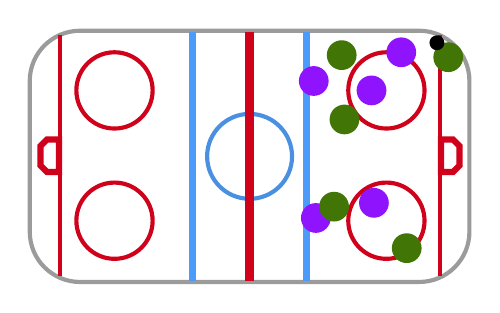
\begin{tikzpicture}[x=0.75pt,y=0.75pt,yscale=-1,xscale=1]
%uncomment if require: \path (0,128.3333282470703); %set diagram left start at 0, and has height of 128.3333282470703

%Rounded Rect [id:dp38410123205883884] 
\draw  [color={rgb, 255:red, 155; green, 155; blue, 155 }  ,draw opacity=1 ][fill={rgb, 255:red, 255; green, 255; blue, 255 }  ,fill opacity=1 ][line width=1.5]  (17,34.16) .. controls (17,20.79) and (27.84,9.95) .. (41.21,9.95) -- (204.62,9.95) .. controls (217.99,9.95) and (228.83,20.79) .. (228.83,34.16) -- (228.83,106.79) .. controls (228.83,120.16) and (217.99,131) .. (204.62,131) -- (41.21,131) .. controls (27.84,131) and (17,120.16) .. (17,106.79) -- cycle ;
%Shape: Circle [id:dp700645285053769] 
\draw  [color={rgb, 255:red, 74; green, 144; blue, 226 }  ,draw opacity=1 ][line width=1.5]  (102.46,70.48) .. controls (102.46,59.18) and (111.62,50.02) .. (122.92,50.02) .. controls (134.22,50.02) and (143.37,59.18) .. (143.37,70.48) .. controls (143.37,81.78) and (134.22,90.93) .. (122.92,90.93) .. controls (111.62,90.93) and (102.46,81.78) .. (102.46,70.48) -- cycle ;
%Shape: Ellipse [id:dp392734969739023] 
\draw  [color={rgb, 255:red, 208; green, 2; blue, 27 }  ,draw opacity=1 ][line width=1.5]  (39.46,38.7) .. controls (39.46,28.56) and (47.68,20.33) .. (57.83,20.33) .. controls (67.97,20.33) and (76.2,28.56) .. (76.2,38.7) .. controls (76.2,48.85) and (67.97,57.07) .. (57.83,57.07) .. controls (47.68,57.07) and (39.46,48.85) .. (39.46,38.7) -- cycle ;
%Shape: Circle [id:dp6100166197818258] 
\draw  [color={rgb, 255:red, 208; green, 2; blue, 27 }  ,draw opacity=1 ][line width=1.5]  (39.46,101.48) .. controls (39.46,91.34) and (47.68,83.11) .. (57.83,83.11) .. controls (67.97,83.11) and (76.2,91.34) .. (76.2,101.48) .. controls (76.2,111.63) and (67.97,119.85) .. (57.83,119.85) .. controls (47.68,119.85) and (39.46,111.63) .. (39.46,101.48) -- cycle ;
%Straight Lines [id:da7658871694895448] 
\draw [color={rgb, 255:red, 76; green, 154; blue, 249 }  ,draw opacity=1 ][line width=2.25]    (95.46,10.48) -- (95.46,130.48) ;


%Straight Lines [id:da7777652289379515] 
\draw [color={rgb, 255:red, 76; green, 154; blue, 249 }  ,draw opacity=1 ][line width=2.25]    (150.37,10.48) -- (150.37,130.48) ;


%Straight Lines [id:da976245400906059] 
\draw [color={rgb, 255:red, 208; green, 2; blue, 27 }  ,draw opacity=1 ][line width=3]    (122.92,10.48) -- (122.92,130.48) ;


%Straight Lines [id:da30486898914991944] 
\draw [color={rgb, 255:red, 208; green, 2; blue, 27 }  ,draw opacity=1 ][line width=1.5]    (214.62,12) -- (214.62,128.33) ;


%Straight Lines [id:da2869662039849248] 
\draw [color={rgb, 255:red, 208; green, 2; blue, 27 }  ,draw opacity=1 ][line width=1.5]    (31.62,12) -- (31.62,128.33) ;


%Snip Same Side Corner Rect [id:dp7059557082920507] 
\draw  [color={rgb, 255:red, 208; green, 2; blue, 27 }  ,draw opacity=1 ][line width=2.25]  (220.96,62.35) -- (224.09,65.48) -- (224.09,74.85) -- (220.96,77.98) -- (215.16,77.98) -- (215.16,77.98) -- (215.16,62.35) -- (215.16,62.35) -- cycle ;
%Snip Same Side Corner Rect [id:dp5407472213865441] 
\draw  [color={rgb, 255:red, 208; green, 2; blue, 27 }  ,draw opacity=1 ][line width=2.25]  (25.28,77.98) -- (22.16,74.85) -- (22.16,65.48) -- (25.28,62.35) -- (31.09,62.35) -- (31.09,62.35) -- (31.09,77.98) -- (31.09,77.98) -- cycle ;
%Shape: Ellipse [id:dp31959491177812605] 
\draw  [color={rgb, 255:red, 208; green, 2; blue, 27 }  ,draw opacity=1 ][line width=1.5]  (170.46,38.7) .. controls (170.46,28.56) and (178.68,20.33) .. (188.83,20.33) .. controls (198.97,20.33) and (207.2,28.56) .. (207.2,38.7) .. controls (207.2,48.85) and (198.97,57.07) .. (188.83,57.07) .. controls (178.68,57.07) and (170.46,48.85) .. (170.46,38.7) -- cycle ;
%Shape: Circle [id:dp7023139486339371] 
\draw  [color={rgb, 255:red, 208; green, 2; blue, 27 }  ,draw opacity=1 ][line width=1.5]  (170.46,101.48) .. controls (170.46,91.34) and (178.68,83.11) .. (188.83,83.11) .. controls (198.97,83.11) and (207.2,91.34) .. (207.2,101.48) .. controls (207.2,111.63) and (198.97,119.85) .. (188.83,119.85) .. controls (178.68,119.85) and (170.46,111.63) .. (170.46,101.48) -- cycle ;

%Shape: Circle [id:dp29979937471102414] 
\draw  [draw opacity=0][fill={rgb, 255:red, 144; green, 19; blue, 254 }  ,fill opacity=1 ] (146.67,34.17) .. controls (146.67,30.21) and (149.88,27) .. (153.83,27) .. controls (157.79,27) and (161,30.21) .. (161,34.17) .. controls (161,38.12) and (157.79,41.33) .. (153.83,41.33) .. controls (149.88,41.33) and (146.67,38.12) .. (146.67,34.17) -- cycle ;
%Shape: Circle [id:dp5829462157157446] 
\draw  [draw opacity=0][fill={rgb, 255:red, 144; green, 19; blue, 254 }  ,fill opacity=1 ] (147.67,100.17) .. controls (147.67,96.21) and (150.88,93) .. (154.83,93) .. controls (158.79,93) and (162,96.21) .. (162,100.17) .. controls (162,104.12) and (158.79,107.33) .. (154.83,107.33) .. controls (150.88,107.33) and (147.67,104.12) .. (147.67,100.17) -- cycle ;
%Shape: Circle [id:dp006696248319188358] 
\draw  [draw opacity=0][fill={rgb, 255:red, 144; green, 19; blue, 254 }  ,fill opacity=1 ] (175.66,92.87) .. controls (175.66,88.91) and (178.87,85.7) .. (182.83,85.7) .. controls (186.79,85.7) and (189.99,88.91) .. (189.99,92.87) .. controls (189.99,96.83) and (186.79,100.04) .. (182.83,100.04) .. controls (178.87,100.04) and (175.66,96.83) .. (175.66,92.87) -- cycle ;
%Shape: Circle [id:dp08943447695410733] 
\draw  [draw opacity=0][fill={rgb, 255:red, 144; green, 19; blue, 254 }  ,fill opacity=1 ] (174.49,38.7) .. controls (174.49,34.74) and (177.7,31.54) .. (181.66,31.54) .. controls (185.62,31.54) and (188.83,34.74) .. (188.83,38.7) .. controls (188.83,42.66) and (185.62,45.87) .. (181.66,45.87) .. controls (177.7,45.87) and (174.49,42.66) .. (174.49,38.7) -- cycle ;
%Shape: Circle [id:dp41233507029199035] 
\draw  [draw opacity=0][fill={rgb, 255:red, 144; green, 19; blue, 254 }  ,fill opacity=1 ] (188.83,20.33) .. controls (188.83,16.38) and (192.04,13.17) .. (195.99,13.17) .. controls (199.95,13.17) and (203.16,16.38) .. (203.16,20.33) .. controls (203.16,24.29) and (199.95,27.5) .. (195.99,27.5) .. controls (192.04,27.5) and (188.83,24.29) .. (188.83,20.33) -- cycle ;
%Shape: Circle [id:dp44417271157090177] 
\draw  [draw opacity=0][fill={rgb, 255:red, 65; green, 117; blue, 5 }  ,fill opacity=1 ] (211.46,22.7) .. controls (211.46,18.74) and (214.67,15.54) .. (218.62,15.54) .. controls (222.58,15.54) and (225.79,18.74) .. (225.79,22.7) .. controls (225.79,26.66) and (222.58,29.87) .. (218.62,29.87) .. controls (214.67,29.87) and (211.46,26.66) .. (211.46,22.7) -- cycle ;
%Shape: Circle [id:dp01396170550742526] 
\draw  [draw opacity=0][fill={rgb, 255:red, 65; green, 117; blue, 5 }  ,fill opacity=1 ] (160.13,21.7) .. controls (160.13,17.74) and (163.33,14.54) .. (167.29,14.54) .. controls (171.25,14.54) and (174.46,17.74) .. (174.46,21.7) .. controls (174.46,25.66) and (171.25,28.87) .. (167.29,28.87) .. controls (163.33,28.87) and (160.13,25.66) .. (160.13,21.7) -- cycle ;
%Shape: Circle [id:dp8789356668978106] 
\draw  [draw opacity=0][fill={rgb, 255:red, 65; green, 117; blue, 5 }  ,fill opacity=1 ] (191.46,114.7) .. controls (191.46,110.74) and (194.67,107.54) .. (198.62,107.54) .. controls (202.58,107.54) and (205.79,110.74) .. (205.79,114.7) .. controls (205.79,118.66) and (202.58,121.87) .. (198.62,121.87) .. controls (194.67,121.87) and (191.46,118.66) .. (191.46,114.7) -- cycle ;
%Shape: Circle [id:dp761516724165991] 
\draw  [draw opacity=0][fill={rgb, 255:red, 65; green, 117; blue, 5 }  ,fill opacity=1 ] (161.46,52.7) .. controls (161.46,48.74) and (164.67,45.54) .. (168.62,45.54) .. controls (172.58,45.54) and (175.79,48.74) .. (175.79,52.7) .. controls (175.79,56.66) and (172.58,59.87) .. (168.62,59.87) .. controls (164.67,59.87) and (161.46,56.66) .. (161.46,52.7) -- cycle ;
%Shape: Circle [id:dp5854423145952716] 
\draw  [draw opacity=0][fill={rgb, 255:red, 65; green, 117; blue, 5 }  ,fill opacity=1 ] (156.46,94.7) .. controls (156.46,90.74) and (159.67,87.54) .. (163.62,87.54) .. controls (167.58,87.54) and (170.79,90.74) .. (170.79,94.7) .. controls (170.79,98.66) and (167.58,101.87) .. (163.62,101.87) .. controls (159.67,101.87) and (156.46,98.66) .. (156.46,94.7) -- cycle ;
%Shape: Circle [id:dp8749898163336198] 
\draw  [draw opacity=0][fill={rgb, 255:red, 0; green, 0; blue, 0 }  ,fill opacity=1 ] (209.58,15.75) .. controls (209.58,13.77) and (211.18,12.17) .. (213.16,12.17) .. controls (215.14,12.17) and (216.74,13.77) .. (216.74,15.75) .. controls (216.74,17.73) and (215.14,19.33) .. (213.16,19.33) .. controls (211.18,19.33) and (209.58,17.73) .. (209.58,15.75) -- cycle ;




\end{tikzpicture}

\end{minipage}

\paragraph{\textcolor{teal}{1-2-2 aggressive}} gives the opponent the least amount of breathing room.

\begin{minipage}{0.4\columnwidth}
\begin{itemize}[leftmargin = *]
	\item	1 forward aggressively deep in the zone.
	\item	2 forwards more aggressive in the zone.
	\item	2 defenders a little closer on the blue line.
\end{itemize}
\end{minipage}
\begin{minipage}{0.6\columnwidth}

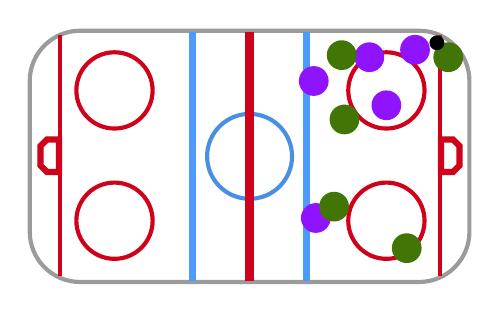
\begin{tikzpicture}[x=0.75pt,y=0.75pt,yscale=-1,xscale=1]
%uncomment if require: \path (0,300); %set diagram left start at 0, and has height of 300

%Rounded Rect [id:dp38410123205883884] 
\draw  [color={rgb, 255:red, 155; green, 155; blue, 155 }  ,draw opacity=1 ][fill={rgb, 255:red, 255; green, 255; blue, 255 }  ,fill opacity=1 ][line width=1.5]  (17,34.16) .. controls (17,20.79) and (27.84,9.95) .. (41.21,9.95) -- (204.62,9.95) .. controls (217.99,9.95) and (228.83,20.79) .. (228.83,34.16) -- (228.83,106.79) .. controls (228.83,120.16) and (217.99,131) .. (204.62,131) -- (41.21,131) .. controls (27.84,131) and (17,120.16) .. (17,106.79) -- cycle ;
%Shape: Circle [id:dp700645285053769] 
\draw  [color={rgb, 255:red, 74; green, 144; blue, 226 }  ,draw opacity=1 ][line width=1.5]  (102.46,70.48) .. controls (102.46,59.18) and (111.62,50.02) .. (122.92,50.02) .. controls (134.22,50.02) and (143.37,59.18) .. (143.37,70.48) .. controls (143.37,81.78) and (134.22,90.93) .. (122.92,90.93) .. controls (111.62,90.93) and (102.46,81.78) .. (102.46,70.48) -- cycle ;
%Shape: Ellipse [id:dp392734969739023] 
\draw  [color={rgb, 255:red, 208; green, 2; blue, 27 }  ,draw opacity=1 ][line width=1.5]  (39.46,38.7) .. controls (39.46,28.56) and (47.68,20.33) .. (57.83,20.33) .. controls (67.97,20.33) and (76.2,28.56) .. (76.2,38.7) .. controls (76.2,48.85) and (67.97,57.07) .. (57.83,57.07) .. controls (47.68,57.07) and (39.46,48.85) .. (39.46,38.7) -- cycle ;
%Shape: Circle [id:dp6100166197818258] 
\draw  [color={rgb, 255:red, 208; green, 2; blue, 27 }  ,draw opacity=1 ][line width=1.5]  (39.46,101.48) .. controls (39.46,91.34) and (47.68,83.11) .. (57.83,83.11) .. controls (67.97,83.11) and (76.2,91.34) .. (76.2,101.48) .. controls (76.2,111.63) and (67.97,119.85) .. (57.83,119.85) .. controls (47.68,119.85) and (39.46,111.63) .. (39.46,101.48) -- cycle ;
%Straight Lines [id:da7658871694895448] 
\draw [color={rgb, 255:red, 76; green, 154; blue, 249 }  ,draw opacity=1 ][line width=2.25]    (95.46,10.48) -- (95.46,130.48) ;


%Straight Lines [id:da7777652289379515] 
\draw [color={rgb, 255:red, 76; green, 154; blue, 249 }  ,draw opacity=1 ][line width=2.25]    (150.37,10.48) -- (150.37,130.48) ;


%Straight Lines [id:da976245400906059] 
\draw [color={rgb, 255:red, 208; green, 2; blue, 27 }  ,draw opacity=1 ][line width=3]    (122.92,10.48) -- (122.92,130.48) ;


%Straight Lines [id:da30486898914991944] 
\draw [color={rgb, 255:red, 208; green, 2; blue, 27 }  ,draw opacity=1 ][line width=1.5]    (214.62,12) -- (214.62,128.33) ;


%Straight Lines [id:da2869662039849248] 
\draw [color={rgb, 255:red, 208; green, 2; blue, 27 }  ,draw opacity=1 ][line width=1.5]    (31.62,12) -- (31.62,128.33) ;


%Snip Same Side Corner Rect [id:dp7059557082920507] 
\draw  [color={rgb, 255:red, 208; green, 2; blue, 27 }  ,draw opacity=1 ][line width=2.25]  (220.96,62.35) -- (224.09,65.48) -- (224.09,74.85) -- (220.96,77.98) -- (215.16,77.98) -- (215.16,77.98) -- (215.16,62.35) -- (215.16,62.35) -- cycle ;
%Snip Same Side Corner Rect [id:dp5407472213865441] 
\draw  [color={rgb, 255:red, 208; green, 2; blue, 27 }  ,draw opacity=1 ][line width=2.25]  (25.28,77.98) -- (22.16,74.85) -- (22.16,65.48) -- (25.28,62.35) -- (31.09,62.35) -- (31.09,62.35) -- (31.09,77.98) -- (31.09,77.98) -- cycle ;
%Shape: Ellipse [id:dp31959491177812605] 
\draw  [color={rgb, 255:red, 208; green, 2; blue, 27 }  ,draw opacity=1 ][line width=1.5]  (170.46,38.7) .. controls (170.46,28.56) and (178.68,20.33) .. (188.83,20.33) .. controls (198.97,20.33) and (207.2,28.56) .. (207.2,38.7) .. controls (207.2,48.85) and (198.97,57.07) .. (188.83,57.07) .. controls (178.68,57.07) and (170.46,48.85) .. (170.46,38.7) -- cycle ;
%Shape: Circle [id:dp7023139486339371] 
\draw  [color={rgb, 255:red, 208; green, 2; blue, 27 }  ,draw opacity=1 ][line width=1.5]  (170.46,101.48) .. controls (170.46,91.34) and (178.68,83.11) .. (188.83,83.11) .. controls (198.97,83.11) and (207.2,91.34) .. (207.2,101.48) .. controls (207.2,111.63) and (198.97,119.85) .. (188.83,119.85) .. controls (178.68,119.85) and (170.46,111.63) .. (170.46,101.48) -- cycle ;

%Shape: Circle [id:dp29979937471102414] 
\draw  [draw opacity=0][fill={rgb, 255:red, 144; green, 19; blue, 254 }  ,fill opacity=1 ] (146.67,34.17) .. controls (146.67,30.21) and (149.88,27) .. (153.83,27) .. controls (157.79,27) and (161,30.21) .. (161,34.17) .. controls (161,38.12) and (157.79,41.33) .. (153.83,41.33) .. controls (149.88,41.33) and (146.67,38.12) .. (146.67,34.17) -- cycle ;
%Shape: Circle [id:dp5829462157157446] 
\draw  [draw opacity=0][fill={rgb, 255:red, 144; green, 19; blue, 254 }  ,fill opacity=1 ] (147.67,100.17) .. controls (147.67,96.21) and (150.88,93) .. (154.83,93) .. controls (158.79,93) and (162,96.21) .. (162,100.17) .. controls (162,104.12) and (158.79,107.33) .. (154.83,107.33) .. controls (150.88,107.33) and (147.67,104.12) .. (147.67,100.17) -- cycle ;
%Shape: Circle [id:dp006696248319188358] 
\draw  [draw opacity=0][fill={rgb, 255:red, 144; green, 19; blue, 254 }  ,fill opacity=1 ] (181.66,45.87) .. controls (181.66,41.91) and (184.87,38.7) .. (188.83,38.7) .. controls (192.79,38.7) and (195.99,41.91) .. (195.99,45.87) .. controls (195.99,49.83) and (192.79,53.04) .. (188.83,53.04) .. controls (184.87,53.04) and (181.66,49.83) .. (181.66,45.87) -- cycle ;
%Shape: Circle [id:dp08943447695410733] 
\draw  [draw opacity=0][fill={rgb, 255:red, 144; green, 19; blue, 254 }  ,fill opacity=1 ] (173.46,22.7) .. controls (173.46,18.74) and (176.67,15.54) .. (180.62,15.54) .. controls (184.58,15.54) and (187.79,18.74) .. (187.79,22.7) .. controls (187.79,26.66) and (184.58,29.87) .. (180.62,29.87) .. controls (176.67,29.87) and (173.46,26.66) .. (173.46,22.7) -- cycle ;
%Shape: Circle [id:dp41233507029199035] 
\draw  [draw opacity=0][fill={rgb, 255:red, 144; green, 19; blue, 254 }  ,fill opacity=1 ] (195.46,19.12) .. controls (195.46,15.16) and (198.67,11.95) .. (202.62,11.95) .. controls (206.58,11.95) and (209.79,15.16) .. (209.79,19.12) .. controls (209.79,23.08) and (206.58,26.29) .. (202.62,26.29) .. controls (198.67,26.29) and (195.46,23.08) .. (195.46,19.12) -- cycle ;
%Shape: Circle [id:dp44417271157090177] 
\draw  [draw opacity=0][fill={rgb, 255:red, 65; green, 117; blue, 5 }  ,fill opacity=1 ] (211.46,22.7) .. controls (211.46,18.74) and (214.67,15.54) .. (218.62,15.54) .. controls (222.58,15.54) and (225.79,18.74) .. (225.79,22.7) .. controls (225.79,26.66) and (222.58,29.87) .. (218.62,29.87) .. controls (214.67,29.87) and (211.46,26.66) .. (211.46,22.7) -- cycle ;
%Shape: Circle [id:dp01396170550742526] 
\draw  [draw opacity=0][fill={rgb, 255:red, 65; green, 117; blue, 5 }  ,fill opacity=1 ] (160.13,21.7) .. controls (160.13,17.74) and (163.33,14.54) .. (167.29,14.54) .. controls (171.25,14.54) and (174.46,17.74) .. (174.46,21.7) .. controls (174.46,25.66) and (171.25,28.87) .. (167.29,28.87) .. controls (163.33,28.87) and (160.13,25.66) .. (160.13,21.7) -- cycle ;
%Shape: Circle [id:dp8789356668978106] 
\draw  [draw opacity=0][fill={rgb, 255:red, 65; green, 117; blue, 5 }  ,fill opacity=1 ] (191.46,114.7) .. controls (191.46,110.74) and (194.67,107.54) .. (198.62,107.54) .. controls (202.58,107.54) and (205.79,110.74) .. (205.79,114.7) .. controls (205.79,118.66) and (202.58,121.87) .. (198.62,121.87) .. controls (194.67,121.87) and (191.46,118.66) .. (191.46,114.7) -- cycle ;
%Shape: Circle [id:dp761516724165991] 
\draw  [draw opacity=0][fill={rgb, 255:red, 65; green, 117; blue, 5 }  ,fill opacity=1 ] (161.46,52.7) .. controls (161.46,48.74) and (164.67,45.54) .. (168.62,45.54) .. controls (172.58,45.54) and (175.79,48.74) .. (175.79,52.7) .. controls (175.79,56.66) and (172.58,59.87) .. (168.62,59.87) .. controls (164.67,59.87) and (161.46,56.66) .. (161.46,52.7) -- cycle ;
%Shape: Circle [id:dp5854423145952716] 
\draw  [draw opacity=0][fill={rgb, 255:red, 65; green, 117; blue, 5 }  ,fill opacity=1 ] (156.46,94.7) .. controls (156.46,90.74) and (159.67,87.54) .. (163.62,87.54) .. controls (167.58,87.54) and (170.79,90.74) .. (170.79,94.7) .. controls (170.79,98.66) and (167.58,101.87) .. (163.62,101.87) .. controls (159.67,101.87) and (156.46,98.66) .. (156.46,94.7) -- cycle ;
%Shape: Circle [id:dp8749898163336198] 
\draw  [draw opacity=0][fill={rgb, 255:red, 0; green, 0; blue, 0 }  ,fill opacity=1 ] (209.58,15.75) .. controls (209.58,13.77) and (211.18,12.17) .. (213.16,12.17) .. controls (215.14,12.17) and (216.74,13.77) .. (216.74,15.75) .. controls (216.74,17.73) and (215.14,19.33) .. (213.16,19.33) .. controls (211.18,19.33) and (209.58,17.73) .. (209.58,15.75) -- cycle ;




\end{tikzpicture}

\end{minipage}

\paragraph{2-3}: 

\begin{minipage}{0.4\columnwidth}
\begin{itemize}[leftmargin = *]
	\item	2 forwards more aggressive in the zone.
	\item	1 forward more passively in the zone.
	\item	2 defenders much further.
\end{itemize}
\end{minipage}
\begin{minipage}{0.6\columnwidth}

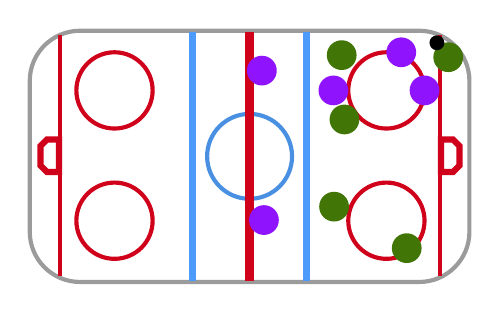
\begin{tikzpicture}[x=0.75pt,y=0.75pt,yscale=-1,xscale=1]
%uncomment if require: \path (0,142.66665649414062); %set diagram left start at 0, and has height of 142.66665649414062

%Rounded Rect [id:dp6258107511117066] 
\draw  [color={rgb, 255:red, 155; green, 155; blue, 155 }  ,draw opacity=1 ][fill={rgb, 255:red, 255; green, 255; blue, 255 }  ,fill opacity=1 ][line width=1.5]  (17,34.16) .. controls (17,20.79) and (27.84,9.95) .. (41.21,9.95) -- (204.62,9.95) .. controls (217.99,9.95) and (228.83,20.79) .. (228.83,34.16) -- (228.83,106.79) .. controls (228.83,120.16) and (217.99,131) .. (204.62,131) -- (41.21,131) .. controls (27.84,131) and (17,120.16) .. (17,106.79) -- cycle ;
%Shape: Circle [id:dp3018457504446248] 
\draw  [color={rgb, 255:red, 74; green, 144; blue, 226 }  ,draw opacity=1 ][line width=1.5]  (102.46,70.48) .. controls (102.46,59.18) and (111.62,50.02) .. (122.92,50.02) .. controls (134.22,50.02) and (143.37,59.18) .. (143.37,70.48) .. controls (143.37,81.78) and (134.22,90.93) .. (122.92,90.93) .. controls (111.62,90.93) and (102.46,81.78) .. (102.46,70.48) -- cycle ;
%Shape: Ellipse [id:dp07466971800950373] 
\draw  [color={rgb, 255:red, 208; green, 2; blue, 27 }  ,draw opacity=1 ][line width=1.5]  (39.46,38.7) .. controls (39.46,28.56) and (47.68,20.33) .. (57.83,20.33) .. controls (67.97,20.33) and (76.2,28.56) .. (76.2,38.7) .. controls (76.2,48.85) and (67.97,57.07) .. (57.83,57.07) .. controls (47.68,57.07) and (39.46,48.85) .. (39.46,38.7) -- cycle ;
%Shape: Circle [id:dp3308444073961254] 
\draw  [color={rgb, 255:red, 208; green, 2; blue, 27 }  ,draw opacity=1 ][line width=1.5]  (39.46,101.48) .. controls (39.46,91.34) and (47.68,83.11) .. (57.83,83.11) .. controls (67.97,83.11) and (76.2,91.34) .. (76.2,101.48) .. controls (76.2,111.63) and (67.97,119.85) .. (57.83,119.85) .. controls (47.68,119.85) and (39.46,111.63) .. (39.46,101.48) -- cycle ;
%Straight Lines [id:da4686331974076998] 
\draw [color={rgb, 255:red, 76; green, 154; blue, 249 }  ,draw opacity=1 ][line width=2.25]    (95.46,10.48) -- (95.46,130.48) ;


%Straight Lines [id:da11020079231172764] 
\draw [color={rgb, 255:red, 76; green, 154; blue, 249 }  ,draw opacity=1 ][line width=2.25]    (150.37,10.48) -- (150.37,130.48) ;


%Straight Lines [id:da2635334919770973] 
\draw [color={rgb, 255:red, 208; green, 2; blue, 27 }  ,draw opacity=1 ][line width=3]    (122.92,10.48) -- (122.92,130.48) ;


%Straight Lines [id:da6116270738771739] 
\draw [color={rgb, 255:red, 208; green, 2; blue, 27 }  ,draw opacity=1 ][line width=1.5]    (214.62,12) -- (214.62,128.33) ;


%Straight Lines [id:da07393178950615886] 
\draw [color={rgb, 255:red, 208; green, 2; blue, 27 }  ,draw opacity=1 ][line width=1.5]    (31.62,12) -- (31.62,128.33) ;


%Snip Same Side Corner Rect [id:dp04583555728641042] 
\draw  [color={rgb, 255:red, 208; green, 2; blue, 27 }  ,draw opacity=1 ][line width=2.25]  (220.96,62.35) -- (224.09,65.48) -- (224.09,74.85) -- (220.96,77.98) -- (215.16,77.98) -- (215.16,77.98) -- (215.16,62.35) -- (215.16,62.35) -- cycle ;
%Snip Same Side Corner Rect [id:dp8006864589098481] 
\draw  [color={rgb, 255:red, 208; green, 2; blue, 27 }  ,draw opacity=1 ][line width=2.25]  (25.28,77.98) -- (22.16,74.85) -- (22.16,65.48) -- (25.28,62.35) -- (31.09,62.35) -- (31.09,62.35) -- (31.09,77.98) -- (31.09,77.98) -- cycle ;
%Shape: Ellipse [id:dp2585703755974025] 
\draw  [color={rgb, 255:red, 208; green, 2; blue, 27 }  ,draw opacity=1 ][line width=1.5]  (170.46,38.7) .. controls (170.46,28.56) and (178.68,20.33) .. (188.83,20.33) .. controls (198.97,20.33) and (207.2,28.56) .. (207.2,38.7) .. controls (207.2,48.85) and (198.97,57.07) .. (188.83,57.07) .. controls (178.68,57.07) and (170.46,48.85) .. (170.46,38.7) -- cycle ;
%Shape: Circle [id:dp6471986972737049] 
\draw  [color={rgb, 255:red, 208; green, 2; blue, 27 }  ,draw opacity=1 ][line width=1.5]  (170.46,101.48) .. controls (170.46,91.34) and (178.68,83.11) .. (188.83,83.11) .. controls (198.97,83.11) and (207.2,91.34) .. (207.2,101.48) .. controls (207.2,111.63) and (198.97,119.85) .. (188.83,119.85) .. controls (178.68,119.85) and (170.46,111.63) .. (170.46,101.48) -- cycle ;

%Shape: Circle [id:dp22961674506792207] 
\draw  [draw opacity=0][fill={rgb, 255:red, 144; green, 19; blue, 254 }  ,fill opacity=1 ] (121.67,29.17) .. controls (121.67,25.21) and (124.88,22) .. (128.83,22) .. controls (132.79,22) and (136,25.21) .. (136,29.17) .. controls (136,33.12) and (132.79,36.33) .. (128.83,36.33) .. controls (124.88,36.33) and (121.67,33.12) .. (121.67,29.17) -- cycle ;
%Shape: Circle [id:dp361708851528006] 
\draw  [draw opacity=0][fill={rgb, 255:red, 144; green, 19; blue, 254 }  ,fill opacity=1 ] (122.67,101.17) .. controls (122.67,97.21) and (125.88,94) .. (129.83,94) .. controls (133.79,94) and (137,97.21) .. (137,101.17) .. controls (137,105.12) and (133.79,108.33) .. (129.83,108.33) .. controls (125.88,108.33) and (122.67,105.12) .. (122.67,101.17) -- cycle ;
%Shape: Circle [id:dp9538471188856912] 
\draw  [draw opacity=0][fill={rgb, 255:red, 144; green, 19; blue, 254 }  ,fill opacity=1 ] (200.03,38.7) .. controls (200.03,34.74) and (203.24,31.54) .. (207.2,31.54) .. controls (211.16,31.54) and (214.36,34.74) .. (214.36,38.7) .. controls (214.36,42.66) and (211.16,45.87) .. (207.2,45.87) .. controls (203.24,45.87) and (200.03,42.66) .. (200.03,38.7) -- cycle ;
%Shape: Circle [id:dp742379199123014] 
\draw  [draw opacity=0][fill={rgb, 255:red, 144; green, 19; blue, 254 }  ,fill opacity=1 ] (156.13,38.7) .. controls (156.13,34.74) and (159.33,31.54) .. (163.29,31.54) .. controls (167.25,31.54) and (170.46,34.74) .. (170.46,38.7) .. controls (170.46,42.66) and (167.25,45.87) .. (163.29,45.87) .. controls (159.33,45.87) and (156.13,42.66) .. (156.13,38.7) -- cycle ;
%Shape: Circle [id:dp7930588131530469] 
\draw  [draw opacity=0][fill={rgb, 255:red, 144; green, 19; blue, 254 }  ,fill opacity=1 ] (188.83,20.33) .. controls (188.83,16.38) and (192.04,13.17) .. (195.99,13.17) .. controls (199.95,13.17) and (203.16,16.38) .. (203.16,20.33) .. controls (203.16,24.29) and (199.95,27.5) .. (195.99,27.5) .. controls (192.04,27.5) and (188.83,24.29) .. (188.83,20.33) -- cycle ;
%Shape: Circle [id:dp049628433650009685] 
\draw  [draw opacity=0][fill={rgb, 255:red, 65; green, 117; blue, 5 }  ,fill opacity=1 ] (211.46,22.7) .. controls (211.46,18.74) and (214.67,15.54) .. (218.62,15.54) .. controls (222.58,15.54) and (225.79,18.74) .. (225.79,22.7) .. controls (225.79,26.66) and (222.58,29.87) .. (218.62,29.87) .. controls (214.67,29.87) and (211.46,26.66) .. (211.46,22.7) -- cycle ;
%Shape: Circle [id:dp5554435595413076] 
\draw  [draw opacity=0][fill={rgb, 255:red, 65; green, 117; blue, 5 }  ,fill opacity=1 ] (160.13,21.7) .. controls (160.13,17.74) and (163.33,14.54) .. (167.29,14.54) .. controls (171.25,14.54) and (174.46,17.74) .. (174.46,21.7) .. controls (174.46,25.66) and (171.25,28.87) .. (167.29,28.87) .. controls (163.33,28.87) and (160.13,25.66) .. (160.13,21.7) -- cycle ;
%Shape: Circle [id:dp03100270285077067] 
\draw  [draw opacity=0][fill={rgb, 255:red, 65; green, 117; blue, 5 }  ,fill opacity=1 ] (191.46,114.7) .. controls (191.46,110.74) and (194.67,107.54) .. (198.62,107.54) .. controls (202.58,107.54) and (205.79,110.74) .. (205.79,114.7) .. controls (205.79,118.66) and (202.58,121.87) .. (198.62,121.87) .. controls (194.67,121.87) and (191.46,118.66) .. (191.46,114.7) -- cycle ;
%Shape: Circle [id:dp24268206581184937] 
\draw  [draw opacity=0][fill={rgb, 255:red, 65; green, 117; blue, 5 }  ,fill opacity=1 ] (161.46,52.7) .. controls (161.46,48.74) and (164.67,45.54) .. (168.62,45.54) .. controls (172.58,45.54) and (175.79,48.74) .. (175.79,52.7) .. controls (175.79,56.66) and (172.58,59.87) .. (168.62,59.87) .. controls (164.67,59.87) and (161.46,56.66) .. (161.46,52.7) -- cycle ;
%Shape: Circle [id:dp3123215987506027] 
\draw  [draw opacity=0][fill={rgb, 255:red, 65; green, 117; blue, 5 }  ,fill opacity=1 ] (156.46,94.7) .. controls (156.46,90.74) and (159.67,87.54) .. (163.62,87.54) .. controls (167.58,87.54) and (170.79,90.74) .. (170.79,94.7) .. controls (170.79,98.66) and (167.58,101.87) .. (163.62,101.87) .. controls (159.67,101.87) and (156.46,98.66) .. (156.46,94.7) -- cycle ;
%Shape: Circle [id:dp3200961501093873] 
\draw  [draw opacity=0][fill={rgb, 255:red, 0; green, 0; blue, 0 }  ,fill opacity=1 ] (209.58,15.75) .. controls (209.58,13.77) and (211.18,12.17) .. (213.16,12.17) .. controls (215.14,12.17) and (216.74,13.77) .. (216.74,15.75) .. controls (216.74,17.73) and (215.14,19.33) .. (213.16,19.33) .. controls (211.18,19.33) and (209.58,17.73) .. (209.58,15.75) -- cycle ;




\end{tikzpicture}

\end{minipage}

\paragraph{Weak Side Lock}: 

\begin{minipage}{0.4\columnwidth}
\begin{itemize}[leftmargin = *]
	\item	Idea is it presses the players onto the board.
\end{itemize}
\end{minipage}
\begin{minipage}{0.6\columnwidth}

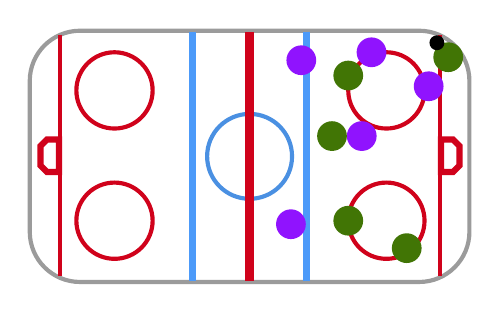
\begin{tikzpicture}[x=0.75pt,y=0.75pt,yscale=-1,xscale=1]
%uncomment if require: \path (0,142.66665649414062); %set diagram left start at 0, and has height of 142.66665649414062

%Rounded Rect [id:dp6258107511117066] 
\draw  [color={rgb, 255:red, 155; green, 155; blue, 155 }  ,draw opacity=1 ][fill={rgb, 255:red, 255; green, 255; blue, 255 }  ,fill opacity=1 ][line width=1.5]  (17,34.16) .. controls (17,20.79) and (27.84,9.95) .. (41.21,9.95) -- (204.62,9.95) .. controls (217.99,9.95) and (228.83,20.79) .. (228.83,34.16) -- (228.83,106.79) .. controls (228.83,120.16) and (217.99,131) .. (204.62,131) -- (41.21,131) .. controls (27.84,131) and (17,120.16) .. (17,106.79) -- cycle ;
%Shape: Circle [id:dp3018457504446248] 
\draw  [color={rgb, 255:red, 74; green, 144; blue, 226 }  ,draw opacity=1 ][line width=1.5]  (102.46,70.48) .. controls (102.46,59.18) and (111.62,50.02) .. (122.92,50.02) .. controls (134.22,50.02) and (143.37,59.18) .. (143.37,70.48) .. controls (143.37,81.78) and (134.22,90.93) .. (122.92,90.93) .. controls (111.62,90.93) and (102.46,81.78) .. (102.46,70.48) -- cycle ;
%Shape: Ellipse [id:dp07466971800950373] 
\draw  [color={rgb, 255:red, 208; green, 2; blue, 27 }  ,draw opacity=1 ][line width=1.5]  (39.46,38.7) .. controls (39.46,28.56) and (47.68,20.33) .. (57.83,20.33) .. controls (67.97,20.33) and (76.2,28.56) .. (76.2,38.7) .. controls (76.2,48.85) and (67.97,57.07) .. (57.83,57.07) .. controls (47.68,57.07) and (39.46,48.85) .. (39.46,38.7) -- cycle ;
%Shape: Circle [id:dp3308444073961254] 
\draw  [color={rgb, 255:red, 208; green, 2; blue, 27 }  ,draw opacity=1 ][line width=1.5]  (39.46,101.48) .. controls (39.46,91.34) and (47.68,83.11) .. (57.83,83.11) .. controls (67.97,83.11) and (76.2,91.34) .. (76.2,101.48) .. controls (76.2,111.63) and (67.97,119.85) .. (57.83,119.85) .. controls (47.68,119.85) and (39.46,111.63) .. (39.46,101.48) -- cycle ;
%Straight Lines [id:da4686331974076998] 
\draw [color={rgb, 255:red, 76; green, 154; blue, 249 }  ,draw opacity=1 ][line width=2.25]    (95.46,10.48) -- (95.46,130.48) ;


%Straight Lines [id:da11020079231172764] 
\draw [color={rgb, 255:red, 76; green, 154; blue, 249 }  ,draw opacity=1 ][line width=2.25]    (150.37,10.48) -- (150.37,130.48) ;


%Straight Lines [id:da2635334919770973] 
\draw [color={rgb, 255:red, 208; green, 2; blue, 27 }  ,draw opacity=1 ][line width=3]    (122.92,10.48) -- (122.92,130.48) ;


%Straight Lines [id:da6116270738771739] 
\draw [color={rgb, 255:red, 208; green, 2; blue, 27 }  ,draw opacity=1 ][line width=1.5]    (214.62,12) -- (214.62,128.33) ;


%Straight Lines [id:da07393178950615886] 
\draw [color={rgb, 255:red, 208; green, 2; blue, 27 }  ,draw opacity=1 ][line width=1.5]    (31.62,12) -- (31.62,128.33) ;


%Snip Same Side Corner Rect [id:dp04583555728641042] 
\draw  [color={rgb, 255:red, 208; green, 2; blue, 27 }  ,draw opacity=1 ][line width=2.25]  (220.96,62.35) -- (224.09,65.48) -- (224.09,74.85) -- (220.96,77.98) -- (215.16,77.98) -- (215.16,77.98) -- (215.16,62.35) -- (215.16,62.35) -- cycle ;
%Snip Same Side Corner Rect [id:dp8006864589098481] 
\draw  [color={rgb, 255:red, 208; green, 2; blue, 27 }  ,draw opacity=1 ][line width=2.25]  (25.28,77.98) -- (22.16,74.85) -- (22.16,65.48) -- (25.28,62.35) -- (31.09,62.35) -- (31.09,62.35) -- (31.09,77.98) -- (31.09,77.98) -- cycle ;
%Shape: Ellipse [id:dp2585703755974025] 
\draw  [color={rgb, 255:red, 208; green, 2; blue, 27 }  ,draw opacity=1 ][line width=1.5]  (170.46,38.7) .. controls (170.46,28.56) and (178.68,20.33) .. (188.83,20.33) .. controls (198.97,20.33) and (207.2,28.56) .. (207.2,38.7) .. controls (207.2,48.85) and (198.97,57.07) .. (188.83,57.07) .. controls (178.68,57.07) and (170.46,48.85) .. (170.46,38.7) -- cycle ;
%Shape: Circle [id:dp6471986972737049] 
\draw  [color={rgb, 255:red, 208; green, 2; blue, 27 }  ,draw opacity=1 ][line width=1.5]  (170.46,101.48) .. controls (170.46,91.34) and (178.68,83.11) .. (188.83,83.11) .. controls (198.97,83.11) and (207.2,91.34) .. (207.2,101.48) .. controls (207.2,111.63) and (198.97,119.85) .. (188.83,119.85) .. controls (178.68,119.85) and (170.46,111.63) .. (170.46,101.48) -- cycle ;

%Shape: Circle [id:dp22961674506792207] 
\draw  [draw opacity=0][fill={rgb, 255:red, 144; green, 19; blue, 254 }  ,fill opacity=1 ] (140.67,24.17) .. controls (140.67,20.21) and (143.88,17) .. (147.83,17) .. controls (151.79,17) and (155,20.21) .. (155,24.17) .. controls (155,28.12) and (151.79,31.33) .. (147.83,31.33) .. controls (143.88,31.33) and (140.67,28.12) .. (140.67,24.17) -- cycle ;
%Shape: Circle [id:dp361708851528006] 
\draw  [draw opacity=0][fill={rgb, 255:red, 144; green, 19; blue, 254 }  ,fill opacity=1 ] (135.67,103.17) .. controls (135.67,99.21) and (138.88,96) .. (142.83,96) .. controls (146.79,96) and (150,99.21) .. (150,103.17) .. controls (150,107.12) and (146.79,110.33) .. (142.83,110.33) .. controls (138.88,110.33) and (135.67,107.12) .. (135.67,103.17) -- cycle ;
%Shape: Circle [id:dp9538471188856912] 
\draw  [draw opacity=0][fill={rgb, 255:red, 144; green, 19; blue, 254 }  ,fill opacity=1 ] (202.03,36.7) .. controls (202.03,32.74) and (205.24,29.54) .. (209.2,29.54) .. controls (213.16,29.54) and (216.36,32.74) .. (216.36,36.7) .. controls (216.36,40.66) and (213.16,43.87) .. (209.2,43.87) .. controls (205.24,43.87) and (202.03,40.66) .. (202.03,36.7) -- cycle ;
%Shape: Circle [id:dp742379199123014] 
\draw  [draw opacity=0][fill={rgb, 255:red, 144; green, 19; blue, 254 }  ,fill opacity=1 ] (169.79,60.7) .. controls (169.79,56.74) and (173,53.54) .. (176.96,53.54) .. controls (180.92,53.54) and (184.12,56.74) .. (184.12,60.7) .. controls (184.12,64.66) and (180.92,67.87) .. (176.96,67.87) .. controls (173,67.87) and (169.79,64.66) .. (169.79,60.7) -- cycle ;
%Shape: Circle [id:dp7930588131530469] 
\draw  [draw opacity=0][fill={rgb, 255:red, 144; green, 19; blue, 254 }  ,fill opacity=1 ] (174.49,20.33) .. controls (174.49,16.38) and (177.7,13.17) .. (181.66,13.17) .. controls (185.62,13.17) and (188.83,16.38) .. (188.83,20.33) .. controls (188.83,24.29) and (185.62,27.5) .. (181.66,27.5) .. controls (177.7,27.5) and (174.49,24.29) .. (174.49,20.33) -- cycle ;
%Shape: Circle [id:dp049628433650009685] 
\draw  [draw opacity=0][fill={rgb, 255:red, 65; green, 117; blue, 5 }  ,fill opacity=1 ] (211.46,22.7) .. controls (211.46,18.74) and (214.67,15.54) .. (218.62,15.54) .. controls (222.58,15.54) and (225.79,18.74) .. (225.79,22.7) .. controls (225.79,26.66) and (222.58,29.87) .. (218.62,29.87) .. controls (214.67,29.87) and (211.46,26.66) .. (211.46,22.7) -- cycle ;
%Shape: Circle [id:dp5554435595413076] 
\draw  [draw opacity=0][fill={rgb, 255:red, 65; green, 117; blue, 5 }  ,fill opacity=1 ] (163.29,31.54) .. controls (163.29,27.58) and (166.5,24.37) .. (170.46,24.37) .. controls (174.42,24.37) and (177.62,27.58) .. (177.62,31.54) .. controls (177.62,35.49) and (174.42,38.7) .. (170.46,38.7) .. controls (166.5,38.7) and (163.29,35.49) .. (163.29,31.54) -- cycle ;
%Shape: Circle [id:dp03100270285077067] 
\draw  [draw opacity=0][fill={rgb, 255:red, 65; green, 117; blue, 5 }  ,fill opacity=1 ] (191.46,114.7) .. controls (191.46,110.74) and (194.67,107.54) .. (198.62,107.54) .. controls (202.58,107.54) and (205.79,110.74) .. (205.79,114.7) .. controls (205.79,118.66) and (202.58,121.87) .. (198.62,121.87) .. controls (194.67,121.87) and (191.46,118.66) .. (191.46,114.7) -- cycle ;
%Shape: Circle [id:dp24268206581184937] 
\draw  [draw opacity=0][fill={rgb, 255:red, 65; green, 117; blue, 5 }  ,fill opacity=1 ] (155.46,60.7) .. controls (155.46,56.74) and (158.67,53.54) .. (162.62,53.54) .. controls (166.58,53.54) and (169.79,56.74) .. (169.79,60.7) .. controls (169.79,64.66) and (166.58,67.87) .. (162.62,67.87) .. controls (158.67,67.87) and (155.46,64.66) .. (155.46,60.7) -- cycle ;
%Shape: Circle [id:dp3123215987506027] 
\draw  [draw opacity=0][fill={rgb, 255:red, 65; green, 117; blue, 5 }  ,fill opacity=1 ] (163.29,101.48) .. controls (163.29,97.52) and (166.5,94.31) .. (170.46,94.31) .. controls (174.42,94.31) and (177.62,97.52) .. (177.62,101.48) .. controls (177.62,105.44) and (174.42,108.65) .. (170.46,108.65) .. controls (166.5,108.65) and (163.29,105.44) .. (163.29,101.48) -- cycle ;
%Shape: Circle [id:dp3200961501093873] 
\draw  [draw opacity=0][fill={rgb, 255:red, 0; green, 0; blue, 0 }  ,fill opacity=1 ] (209.58,15.75) .. controls (209.58,13.77) and (211.18,12.17) .. (213.16,12.17) .. controls (215.14,12.17) and (216.74,13.77) .. (216.74,15.75) .. controls (216.74,17.73) and (215.14,19.33) .. (213.16,19.33) .. controls (211.18,19.33) and (209.58,17.73) .. (209.58,15.75) -- cycle ;




\end{tikzpicture}

\end{minipage}

\subsection*{Neutral Zone} Position of players when the opponent gets the puck out of their zone and into center ice.

\paragraph{\textcolor{teal}{1-3-1}} best against skilled players because the one guy in the back prevents the opponent from getting breakaways. 

\begin{minipage}{0.4\columnwidth}
\begin{itemize}[leftmargin = *]
	\item	1 forward pressuring the puck carrier.
	\item	3 players forming a line in the middle to block entry points.
	\item	1 player hanging back in case a player gets through \textbf{OR} he needs to retrieve a puck in case of a dump and chase.
\end{itemize}
\end{minipage}
\begin{minipage}{0.6\columnwidth}

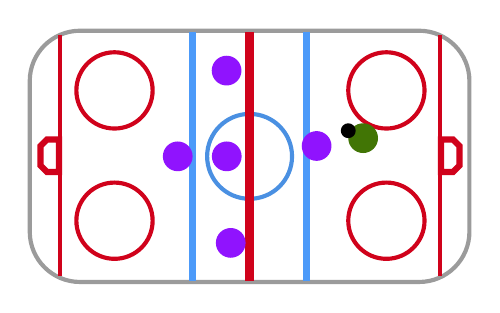
\begin{tikzpicture}[x=0.75pt,y=0.75pt,yscale=-1,xscale=1]
%uncomment if require: \path (0,142.66665649414062); %set diagram left start at 0, and has height of 142.66665649414062

%Rounded Rect [id:dp6258107511117066] 
\draw  [color={rgb, 255:red, 155; green, 155; blue, 155 }  ,draw opacity=1 ][fill={rgb, 255:red, 255; green, 255; blue, 255 }  ,fill opacity=1 ][line width=1.5]  (17,34.16) .. controls (17,20.79) and (27.84,9.95) .. (41.21,9.95) -- (204.62,9.95) .. controls (217.99,9.95) and (228.83,20.79) .. (228.83,34.16) -- (228.83,106.79) .. controls (228.83,120.16) and (217.99,131) .. (204.62,131) -- (41.21,131) .. controls (27.84,131) and (17,120.16) .. (17,106.79) -- cycle ;
%Shape: Circle [id:dp3018457504446248] 
\draw  [color={rgb, 255:red, 74; green, 144; blue, 226 }  ,draw opacity=1 ][line width=1.5]  (102.46,70.48) .. controls (102.46,59.18) and (111.62,50.02) .. (122.92,50.02) .. controls (134.22,50.02) and (143.37,59.18) .. (143.37,70.48) .. controls (143.37,81.78) and (134.22,90.93) .. (122.92,90.93) .. controls (111.62,90.93) and (102.46,81.78) .. (102.46,70.48) -- cycle ;
%Shape: Ellipse [id:dp07466971800950373] 
\draw  [color={rgb, 255:red, 208; green, 2; blue, 27 }  ,draw opacity=1 ][line width=1.5]  (39.46,38.7) .. controls (39.46,28.56) and (47.68,20.33) .. (57.83,20.33) .. controls (67.97,20.33) and (76.2,28.56) .. (76.2,38.7) .. controls (76.2,48.85) and (67.97,57.07) .. (57.83,57.07) .. controls (47.68,57.07) and (39.46,48.85) .. (39.46,38.7) -- cycle ;
%Shape: Circle [id:dp3308444073961254] 
\draw  [color={rgb, 255:red, 208; green, 2; blue, 27 }  ,draw opacity=1 ][line width=1.5]  (39.46,101.48) .. controls (39.46,91.34) and (47.68,83.11) .. (57.83,83.11) .. controls (67.97,83.11) and (76.2,91.34) .. (76.2,101.48) .. controls (76.2,111.63) and (67.97,119.85) .. (57.83,119.85) .. controls (47.68,119.85) and (39.46,111.63) .. (39.46,101.48) -- cycle ;
%Straight Lines [id:da4686331974076998] 
\draw [color={rgb, 255:red, 76; green, 154; blue, 249 }  ,draw opacity=1 ][line width=2.25]    (95.46,10.48) -- (95.46,130.48) ;


%Straight Lines [id:da11020079231172764] 
\draw [color={rgb, 255:red, 76; green, 154; blue, 249 }  ,draw opacity=1 ][line width=2.25]    (150.37,10.48) -- (150.37,130.48) ;


%Straight Lines [id:da2635334919770973] 
\draw [color={rgb, 255:red, 208; green, 2; blue, 27 }  ,draw opacity=1 ][line width=3]    (122.92,10.48) -- (122.92,130.48) ;


%Straight Lines [id:da6116270738771739] 
\draw [color={rgb, 255:red, 208; green, 2; blue, 27 }  ,draw opacity=1 ][line width=1.5]    (214.62,12) -- (214.62,128.33) ;


%Straight Lines [id:da07393178950615886] 
\draw [color={rgb, 255:red, 208; green, 2; blue, 27 }  ,draw opacity=1 ][line width=1.5]    (31.62,12) -- (31.62,128.33) ;


%Snip Same Side Corner Rect [id:dp04583555728641042] 
\draw  [color={rgb, 255:red, 208; green, 2; blue, 27 }  ,draw opacity=1 ][line width=2.25]  (220.96,62.35) -- (224.09,65.48) -- (224.09,74.85) -- (220.96,77.98) -- (215.16,77.98) -- (215.16,77.98) -- (215.16,62.35) -- (215.16,62.35) -- cycle ;
%Snip Same Side Corner Rect [id:dp8006864589098481] 
\draw  [color={rgb, 255:red, 208; green, 2; blue, 27 }  ,draw opacity=1 ][line width=2.25]  (25.28,77.98) -- (22.16,74.85) -- (22.16,65.48) -- (25.28,62.35) -- (31.09,62.35) -- (31.09,62.35) -- (31.09,77.98) -- (31.09,77.98) -- cycle ;
%Shape: Ellipse [id:dp2585703755974025] 
\draw  [color={rgb, 255:red, 208; green, 2; blue, 27 }  ,draw opacity=1 ][line width=1.5]  (170.46,38.7) .. controls (170.46,28.56) and (178.68,20.33) .. (188.83,20.33) .. controls (198.97,20.33) and (207.2,28.56) .. (207.2,38.7) .. controls (207.2,48.85) and (198.97,57.07) .. (188.83,57.07) .. controls (178.68,57.07) and (170.46,48.85) .. (170.46,38.7) -- cycle ;
%Shape: Circle [id:dp6471986972737049] 
\draw  [color={rgb, 255:red, 208; green, 2; blue, 27 }  ,draw opacity=1 ][line width=1.5]  (170.46,101.48) .. controls (170.46,91.34) and (178.68,83.11) .. (188.83,83.11) .. controls (198.97,83.11) and (207.2,91.34) .. (207.2,101.48) .. controls (207.2,111.63) and (198.97,119.85) .. (188.83,119.85) .. controls (178.68,119.85) and (170.46,111.63) .. (170.46,101.48) -- cycle ;

%Shape: Circle [id:dp22961674506792207] 
\draw  [draw opacity=0][fill={rgb, 255:red, 144; green, 19; blue, 254 }  ,fill opacity=1 ] (104.67,29.17) .. controls (104.67,25.21) and (107.88,22) .. (111.83,22) .. controls (115.79,22) and (119,25.21) .. (119,29.17) .. controls (119,33.12) and (115.79,36.33) .. (111.83,36.33) .. controls (107.88,36.33) and (104.67,33.12) .. (104.67,29.17) -- cycle ;
%Shape: Circle [id:dp361708851528006] 
\draw  [draw opacity=0][fill={rgb, 255:red, 144; green, 19; blue, 254 }  ,fill opacity=1 ] (106.67,112.17) .. controls (106.67,108.21) and (109.88,105) .. (113.83,105) .. controls (117.79,105) and (121,108.21) .. (121,112.17) .. controls (121,116.12) and (117.79,119.33) .. (113.83,119.33) .. controls (109.88,119.33) and (106.67,116.12) .. (106.67,112.17) -- cycle ;
%Shape: Circle [id:dp9538471188856912] 
\draw  [draw opacity=0][fill={rgb, 255:red, 144; green, 19; blue, 254 }  ,fill opacity=1 ] (148.04,65.48) .. controls (148.04,61.52) and (151.25,58.31) .. (155.21,58.31) .. controls (159.17,58.31) and (162.37,61.52) .. (162.37,65.48) .. controls (162.37,69.43) and (159.17,72.64) .. (155.21,72.64) .. controls (151.25,72.64) and (148.04,69.43) .. (148.04,65.48) -- cycle ;
%Shape: Circle [id:dp742379199123014] 
\draw  [draw opacity=0][fill={rgb, 255:red, 144; green, 19; blue, 254 }  ,fill opacity=1 ] (81.13,70.48) .. controls (81.13,66.52) and (84.33,63.31) .. (88.29,63.31) .. controls (92.25,63.31) and (95.46,66.52) .. (95.46,70.48) .. controls (95.46,74.43) and (92.25,77.64) .. (88.29,77.64) .. controls (84.33,77.64) and (81.13,74.43) .. (81.13,70.48) -- cycle ;
%Shape: Circle [id:dp7930588131530469] 
\draw  [draw opacity=0][fill={rgb, 255:red, 144; green, 19; blue, 254 }  ,fill opacity=1 ] (104.75,70.48) .. controls (104.75,66.52) and (107.96,63.31) .. (111.92,63.31) .. controls (115.87,63.31) and (119.08,66.52) .. (119.08,70.48) .. controls (119.08,74.43) and (115.87,77.64) .. (111.92,77.64) .. controls (107.96,77.64) and (104.75,74.43) .. (104.75,70.48) -- cycle ;
%Shape: Circle [id:dp049628433650009685] 
\draw  [draw opacity=0][fill={rgb, 255:red, 65; green, 117; blue, 5 }  ,fill opacity=1 ] (170.46,61.7) .. controls (170.46,57.74) and (173.67,54.54) .. (177.62,54.54) .. controls (181.58,54.54) and (184.79,57.74) .. (184.79,61.7) .. controls (184.79,65.66) and (181.58,68.87) .. (177.62,68.87) .. controls (173.67,68.87) and (170.46,65.66) .. (170.46,61.7) -- cycle ;
%Shape: Circle [id:dp3200961501093873] 
\draw  [draw opacity=0][fill={rgb, 255:red, 0; green, 0; blue, 0 }  ,fill opacity=1 ] (166.88,58.12) .. controls (166.88,56.14) and (168.48,54.54) .. (170.46,54.54) .. controls (172.44,54.54) and (174.04,56.14) .. (174.04,58.12) .. controls (174.04,60.1) and (172.44,61.7) .. (170.46,61.7) .. controls (168.48,61.7) and (166.88,60.1) .. (166.88,58.12) -- cycle ;




\end{tikzpicture}
\end{minipage}

\paragraph{1-4} Good for beginners and playing against the AI as it's very difficult for the opponent to enter the zone.

\begin{minipage}{0.4\columnwidth}
\begin{itemize}[leftmargin = *]
	\item	1 forward pressuring the puck carrier.
	\item	4 players forming a line on the blue line to block entry.
\end{itemize}
\end{minipage}
\begin{minipage}{0.6\columnwidth}

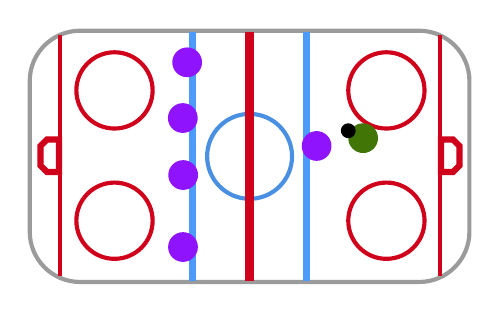
\begin{tikzpicture}[x=0.75pt,y=0.75pt,yscale=-1,xscale=1]
%uncomment if require: \path (0,142.66665649414062); %set diagram left start at 0, and has height of 142.66665649414062

%Rounded Rect [id:dp6258107511117066] 
\draw  [color={rgb, 255:red, 155; green, 155; blue, 155 }  ,draw opacity=1 ][fill={rgb, 255:red, 255; green, 255; blue, 255 }  ,fill opacity=1 ][line width=1.5]  (17,34.16) .. controls (17,20.79) and (27.84,9.95) .. (41.21,9.95) -- (204.62,9.95) .. controls (217.99,9.95) and (228.83,20.79) .. (228.83,34.16) -- (228.83,106.79) .. controls (228.83,120.16) and (217.99,131) .. (204.62,131) -- (41.21,131) .. controls (27.84,131) and (17,120.16) .. (17,106.79) -- cycle ;
%Shape: Circle [id:dp3018457504446248] 
\draw  [color={rgb, 255:red, 74; green, 144; blue, 226 }  ,draw opacity=1 ][line width=1.5]  (102.46,70.48) .. controls (102.46,59.18) and (111.62,50.02) .. (122.92,50.02) .. controls (134.22,50.02) and (143.37,59.18) .. (143.37,70.48) .. controls (143.37,81.78) and (134.22,90.93) .. (122.92,90.93) .. controls (111.62,90.93) and (102.46,81.78) .. (102.46,70.48) -- cycle ;
%Shape: Ellipse [id:dp07466971800950373] 
\draw  [color={rgb, 255:red, 208; green, 2; blue, 27 }  ,draw opacity=1 ][line width=1.5]  (39.46,38.7) .. controls (39.46,28.56) and (47.68,20.33) .. (57.83,20.33) .. controls (67.97,20.33) and (76.2,28.56) .. (76.2,38.7) .. controls (76.2,48.85) and (67.97,57.07) .. (57.83,57.07) .. controls (47.68,57.07) and (39.46,48.85) .. (39.46,38.7) -- cycle ;
%Shape: Circle [id:dp3308444073961254] 
\draw  [color={rgb, 255:red, 208; green, 2; blue, 27 }  ,draw opacity=1 ][line width=1.5]  (39.46,101.48) .. controls (39.46,91.34) and (47.68,83.11) .. (57.83,83.11) .. controls (67.97,83.11) and (76.2,91.34) .. (76.2,101.48) .. controls (76.2,111.63) and (67.97,119.85) .. (57.83,119.85) .. controls (47.68,119.85) and (39.46,111.63) .. (39.46,101.48) -- cycle ;
%Straight Lines [id:da4686331974076998] 
\draw [color={rgb, 255:red, 76; green, 154; blue, 249 }  ,draw opacity=1 ][line width=2.25]    (95.46,10.48) -- (95.46,130.48) ;


%Straight Lines [id:da11020079231172764] 
\draw [color={rgb, 255:red, 76; green, 154; blue, 249 }  ,draw opacity=1 ][line width=2.25]    (150.37,10.48) -- (150.37,130.48) ;


%Straight Lines [id:da2635334919770973] 
\draw [color={rgb, 255:red, 208; green, 2; blue, 27 }  ,draw opacity=1 ][line width=3]    (122.92,10.48) -- (122.92,130.48) ;


%Straight Lines [id:da6116270738771739] 
\draw [color={rgb, 255:red, 208; green, 2; blue, 27 }  ,draw opacity=1 ][line width=1.5]    (214.62,12) -- (214.62,128.33) ;


%Straight Lines [id:da07393178950615886] 
\draw [color={rgb, 255:red, 208; green, 2; blue, 27 }  ,draw opacity=1 ][line width=1.5]    (31.62,12) -- (31.62,128.33) ;


%Snip Same Side Corner Rect [id:dp04583555728641042] 
\draw  [color={rgb, 255:red, 208; green, 2; blue, 27 }  ,draw opacity=1 ][line width=2.25]  (220.96,62.35) -- (224.09,65.48) -- (224.09,74.85) -- (220.96,77.98) -- (215.16,77.98) -- (215.16,77.98) -- (215.16,62.35) -- (215.16,62.35) -- cycle ;
%Snip Same Side Corner Rect [id:dp8006864589098481] 
\draw  [color={rgb, 255:red, 208; green, 2; blue, 27 }  ,draw opacity=1 ][line width=2.25]  (25.28,77.98) -- (22.16,74.85) -- (22.16,65.48) -- (25.28,62.35) -- (31.09,62.35) -- (31.09,62.35) -- (31.09,77.98) -- (31.09,77.98) -- cycle ;
%Shape: Ellipse [id:dp2585703755974025] 
\draw  [color={rgb, 255:red, 208; green, 2; blue, 27 }  ,draw opacity=1 ][line width=1.5]  (170.46,38.7) .. controls (170.46,28.56) and (178.68,20.33) .. (188.83,20.33) .. controls (198.97,20.33) and (207.2,28.56) .. (207.2,38.7) .. controls (207.2,48.85) and (198.97,57.07) .. (188.83,57.07) .. controls (178.68,57.07) and (170.46,48.85) .. (170.46,38.7) -- cycle ;
%Shape: Circle [id:dp6471986972737049] 
\draw  [color={rgb, 255:red, 208; green, 2; blue, 27 }  ,draw opacity=1 ][line width=1.5]  (170.46,101.48) .. controls (170.46,91.34) and (178.68,83.11) .. (188.83,83.11) .. controls (198.97,83.11) and (207.2,91.34) .. (207.2,101.48) .. controls (207.2,111.63) and (198.97,119.85) .. (188.83,119.85) .. controls (178.68,119.85) and (170.46,111.63) .. (170.46,101.48) -- cycle ;

%Shape: Circle [id:dp22961674506792207] 
\draw  [draw opacity=0][fill={rgb, 255:red, 144; green, 19; blue, 254 }  ,fill opacity=1 ] (85.67,25.17) .. controls (85.67,21.21) and (88.88,18) .. (92.83,18) .. controls (96.79,18) and (100,21.21) .. (100,25.17) .. controls (100,29.12) and (96.79,32.33) .. (92.83,32.33) .. controls (88.88,32.33) and (85.67,29.12) .. (85.67,25.17) -- cycle ;
%Shape: Circle [id:dp361708851528006] 
\draw  [draw opacity=0][fill={rgb, 255:red, 144; green, 19; blue, 254 }  ,fill opacity=1 ] (83.67,114.17) .. controls (83.67,110.21) and (86.88,107) .. (90.83,107) .. controls (94.79,107) and (98,110.21) .. (98,114.17) .. controls (98,118.12) and (94.79,121.33) .. (90.83,121.33) .. controls (86.88,121.33) and (83.67,118.12) .. (83.67,114.17) -- cycle ;
%Shape: Circle [id:dp9538471188856912] 
\draw  [draw opacity=0][fill={rgb, 255:red, 144; green, 19; blue, 254 }  ,fill opacity=1 ] (148.04,65.48) .. controls (148.04,61.52) and (151.25,58.31) .. (155.21,58.31) .. controls (159.17,58.31) and (162.37,61.52) .. (162.37,65.48) .. controls (162.37,69.43) and (159.17,72.64) .. (155.21,72.64) .. controls (151.25,72.64) and (148.04,69.43) .. (148.04,65.48) -- cycle ;
%Shape: Circle [id:dp742379199123014] 
\draw  [draw opacity=0][fill={rgb, 255:red, 144; green, 19; blue, 254 }  ,fill opacity=1 ] (83.58,52.02) .. controls (83.58,48.06) and (86.79,44.85) .. (90.75,44.85) .. controls (94.71,44.85) and (97.92,48.06) .. (97.92,52.02) .. controls (97.92,55.98) and (94.71,59.18) .. (90.75,59.18) .. controls (86.79,59.18) and (83.58,55.98) .. (83.58,52.02) -- cycle ;
%Shape: Circle [id:dp7930588131530469] 
\draw  [draw opacity=0][fill={rgb, 255:red, 144; green, 19; blue, 254 }  ,fill opacity=1 ] (83.75,79.48) .. controls (83.75,75.52) and (86.96,72.31) .. (90.92,72.31) .. controls (94.87,72.31) and (98.08,75.52) .. (98.08,79.48) .. controls (98.08,83.43) and (94.87,86.64) .. (90.92,86.64) .. controls (86.96,86.64) and (83.75,83.43) .. (83.75,79.48) -- cycle ;
%Shape: Circle [id:dp049628433650009685] 
\draw  [draw opacity=0][fill={rgb, 255:red, 65; green, 117; blue, 5 }  ,fill opacity=1 ] (170.46,61.7) .. controls (170.46,57.74) and (173.67,54.54) .. (177.62,54.54) .. controls (181.58,54.54) and (184.79,57.74) .. (184.79,61.7) .. controls (184.79,65.66) and (181.58,68.87) .. (177.62,68.87) .. controls (173.67,68.87) and (170.46,65.66) .. (170.46,61.7) -- cycle ;
%Shape: Circle [id:dp3200961501093873] 
\draw  [draw opacity=0][fill={rgb, 255:red, 0; green, 0; blue, 0 }  ,fill opacity=1 ] (166.88,58.12) .. controls (166.88,56.14) and (168.48,54.54) .. (170.46,54.54) .. controls (172.44,54.54) and (174.04,56.14) .. (174.04,58.12) .. controls (174.04,60.1) and (172.44,61.7) .. (170.46,61.7) .. controls (168.48,61.7) and (166.88,60.1) .. (166.88,58.12) -- cycle ;




\end{tikzpicture}

\end{minipage}

\paragraph{1-2-2 Red} Like having a bunch of obstacles in the neutral zone the opponent has to get through. Problem is that with one quick breakout pass the opponent will get through most of your players.

\begin{minipage}{0.4\columnwidth}
\begin{itemize}[leftmargin = *]
	\item	1 forward pressuring the puck.
	\item	2 forwards sit on the red line.
	\item	2 defenders sit on your blue line.
\end{itemize}
\end{minipage}
\begin{minipage}{0.6\columnwidth}

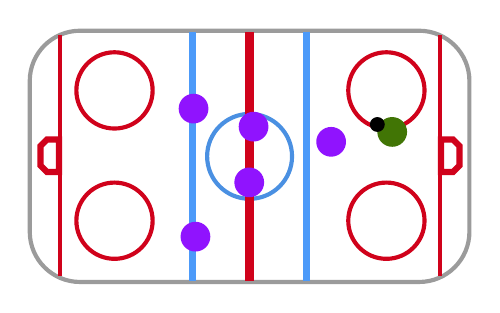
\begin{tikzpicture}[x=0.75pt,y=0.75pt,yscale=-1,xscale=1]
%uncomment if require: \path (0,142.66665649414062); %set diagram left start at 0, and has height of 142.66665649414062

%Rounded Rect [id:dp6258107511117066] 
\draw  [color={rgb, 255:red, 155; green, 155; blue, 155 }  ,draw opacity=1 ][fill={rgb, 255:red, 255; green, 255; blue, 255 }  ,fill opacity=1 ][line width=1.5]  (17,34.16) .. controls (17,20.79) and (27.84,9.95) .. (41.21,9.95) -- (204.62,9.95) .. controls (217.99,9.95) and (228.83,20.79) .. (228.83,34.16) -- (228.83,106.79) .. controls (228.83,120.16) and (217.99,131) .. (204.62,131) -- (41.21,131) .. controls (27.84,131) and (17,120.16) .. (17,106.79) -- cycle ;
%Shape: Circle [id:dp3018457504446248] 
\draw  [color={rgb, 255:red, 74; green, 144; blue, 226 }  ,draw opacity=1 ][line width=1.5]  (102.46,70.48) .. controls (102.46,59.18) and (111.62,50.02) .. (122.92,50.02) .. controls (134.22,50.02) and (143.37,59.18) .. (143.37,70.48) .. controls (143.37,81.78) and (134.22,90.93) .. (122.92,90.93) .. controls (111.62,90.93) and (102.46,81.78) .. (102.46,70.48) -- cycle ;
%Shape: Ellipse [id:dp07466971800950373] 
\draw  [color={rgb, 255:red, 208; green, 2; blue, 27 }  ,draw opacity=1 ][line width=1.5]  (39.46,38.7) .. controls (39.46,28.56) and (47.68,20.33) .. (57.83,20.33) .. controls (67.97,20.33) and (76.2,28.56) .. (76.2,38.7) .. controls (76.2,48.85) and (67.97,57.07) .. (57.83,57.07) .. controls (47.68,57.07) and (39.46,48.85) .. (39.46,38.7) -- cycle ;
%Shape: Circle [id:dp3308444073961254] 
\draw  [color={rgb, 255:red, 208; green, 2; blue, 27 }  ,draw opacity=1 ][line width=1.5]  (39.46,101.48) .. controls (39.46,91.34) and (47.68,83.11) .. (57.83,83.11) .. controls (67.97,83.11) and (76.2,91.34) .. (76.2,101.48) .. controls (76.2,111.63) and (67.97,119.85) .. (57.83,119.85) .. controls (47.68,119.85) and (39.46,111.63) .. (39.46,101.48) -- cycle ;
%Straight Lines [id:da4686331974076998] 
\draw [color={rgb, 255:red, 76; green, 154; blue, 249 }  ,draw opacity=1 ][line width=2.25]    (95.46,10.48) -- (95.46,130.48) ;


%Straight Lines [id:da11020079231172764] 
\draw [color={rgb, 255:red, 76; green, 154; blue, 249 }  ,draw opacity=1 ][line width=2.25]    (150.37,10.48) -- (150.37,130.48) ;


%Straight Lines [id:da2635334919770973] 
\draw [color={rgb, 255:red, 208; green, 2; blue, 27 }  ,draw opacity=1 ][line width=3]    (122.92,10.48) -- (122.92,130.48) ;


%Straight Lines [id:da6116270738771739] 
\draw [color={rgb, 255:red, 208; green, 2; blue, 27 }  ,draw opacity=1 ][line width=1.5]    (214.62,12) -- (214.62,128.33) ;


%Straight Lines [id:da07393178950615886] 
\draw [color={rgb, 255:red, 208; green, 2; blue, 27 }  ,draw opacity=1 ][line width=1.5]    (31.62,12) -- (31.62,128.33) ;


%Snip Same Side Corner Rect [id:dp04583555728641042] 
\draw  [color={rgb, 255:red, 208; green, 2; blue, 27 }  ,draw opacity=1 ][line width=2.25]  (220.96,62.35) -- (224.09,65.48) -- (224.09,74.85) -- (220.96,77.98) -- (215.16,77.98) -- (215.16,77.98) -- (215.16,62.35) -- (215.16,62.35) -- cycle ;
%Snip Same Side Corner Rect [id:dp8006864589098481] 
\draw  [color={rgb, 255:red, 208; green, 2; blue, 27 }  ,draw opacity=1 ][line width=2.25]  (25.28,77.98) -- (22.16,74.85) -- (22.16,65.48) -- (25.28,62.35) -- (31.09,62.35) -- (31.09,62.35) -- (31.09,77.98) -- (31.09,77.98) -- cycle ;
%Shape: Ellipse [id:dp2585703755974025] 
\draw  [color={rgb, 255:red, 208; green, 2; blue, 27 }  ,draw opacity=1 ][line width=1.5]  (170.46,38.7) .. controls (170.46,28.56) and (178.68,20.33) .. (188.83,20.33) .. controls (198.97,20.33) and (207.2,28.56) .. (207.2,38.7) .. controls (207.2,48.85) and (198.97,57.07) .. (188.83,57.07) .. controls (178.68,57.07) and (170.46,48.85) .. (170.46,38.7) -- cycle ;
%Shape: Circle [id:dp6471986972737049] 
\draw  [color={rgb, 255:red, 208; green, 2; blue, 27 }  ,draw opacity=1 ][line width=1.5]  (170.46,101.48) .. controls (170.46,91.34) and (178.68,83.11) .. (188.83,83.11) .. controls (198.97,83.11) and (207.2,91.34) .. (207.2,101.48) .. controls (207.2,111.63) and (198.97,119.85) .. (188.83,119.85) .. controls (178.68,119.85) and (170.46,111.63) .. (170.46,101.48) -- cycle ;

%Shape: Circle [id:dp22961674506792207] 
\draw  [draw opacity=0][fill={rgb, 255:red, 144; green, 19; blue, 254 }  ,fill opacity=1 ] (117.67,56.17) .. controls (117.67,52.21) and (120.88,49) .. (124.83,49) .. controls (128.79,49) and (132,52.21) .. (132,56.17) .. controls (132,60.12) and (128.79,63.33) .. (124.83,63.33) .. controls (120.88,63.33) and (117.67,60.12) .. (117.67,56.17) -- cycle ;
%Shape: Circle [id:dp361708851528006] 
\draw  [draw opacity=0][fill={rgb, 255:red, 144; green, 19; blue, 254 }  ,fill opacity=1 ] (89.67,109.17) .. controls (89.67,105.21) and (92.88,102) .. (96.83,102) .. controls (100.79,102) and (104,105.21) .. (104,109.17) .. controls (104,113.12) and (100.79,116.33) .. (96.83,116.33) .. controls (92.88,116.33) and (89.67,113.12) .. (89.67,109.17) -- cycle ;
%Shape: Circle [id:dp9538471188856912] 
\draw  [draw opacity=0][fill={rgb, 255:red, 144; green, 19; blue, 254 }  ,fill opacity=1 ] (155.04,63.48) .. controls (155.04,59.52) and (158.25,56.31) .. (162.21,56.31) .. controls (166.17,56.31) and (169.37,59.52) .. (169.37,63.48) .. controls (169.37,67.43) and (166.17,70.64) .. (162.21,70.64) .. controls (158.25,70.64) and (155.04,67.43) .. (155.04,63.48) -- cycle ;
%Shape: Circle [id:dp742379199123014] 
\draw  [draw opacity=0][fill={rgb, 255:red, 144; green, 19; blue, 254 }  ,fill opacity=1 ] (115.58,83.02) .. controls (115.58,79.06) and (118.79,75.85) .. (122.75,75.85) .. controls (126.71,75.85) and (129.92,79.06) .. (129.92,83.02) .. controls (129.92,86.98) and (126.71,90.18) .. (122.75,90.18) .. controls (118.79,90.18) and (115.58,86.98) .. (115.58,83.02) -- cycle ;
%Shape: Circle [id:dp7930588131530469] 
\draw  [draw opacity=0][fill={rgb, 255:red, 144; green, 19; blue, 254 }  ,fill opacity=1 ] (88.75,47.48) .. controls (88.75,43.52) and (91.96,40.31) .. (95.92,40.31) .. controls (99.87,40.31) and (103.08,43.52) .. (103.08,47.48) .. controls (103.08,51.43) and (99.87,54.64) .. (95.92,54.64) .. controls (91.96,54.64) and (88.75,51.43) .. (88.75,47.48) -- cycle ;
%Shape: Circle [id:dp049628433650009685] 
\draw  [draw opacity=0][fill={rgb, 255:red, 65; green, 117; blue, 5 }  ,fill opacity=1 ] (184.46,58.7) .. controls (184.46,54.74) and (187.67,51.54) .. (191.62,51.54) .. controls (195.58,51.54) and (198.79,54.74) .. (198.79,58.7) .. controls (198.79,62.66) and (195.58,65.87) .. (191.62,65.87) .. controls (187.67,65.87) and (184.46,62.66) .. (184.46,58.7) -- cycle ;
%Shape: Circle [id:dp3200961501093873] 
\draw  [draw opacity=0][fill={rgb, 255:red, 0; green, 0; blue, 0 }  ,fill opacity=1 ] (180.88,55.12) .. controls (180.88,53.14) and (182.48,51.54) .. (184.46,51.54) .. controls (186.44,51.54) and (188.04,53.14) .. (188.04,55.12) .. controls (188.04,57.1) and (186.44,58.7) .. (184.46,58.7) .. controls (182.48,58.7) and (180.88,57.1) .. (180.88,55.12) -- cycle ;




\end{tikzpicture}
\end{minipage}

\paragraph{1-2-2 Blue}: More aggressive version of 1-2-2 Red. The forwards can then get in on the play if need be.

\begin{minipage}{0.4\columnwidth}
\begin{itemize}[leftmargin = *]
	\item	1 forward pressuring the puck carrier.
	\item	2 forwards pressuring on the blue line.
	\item	2 defenders sit on your red line.
\end{itemize}
\end{minipage}
\begin{minipage}{0.6\columnwidth}

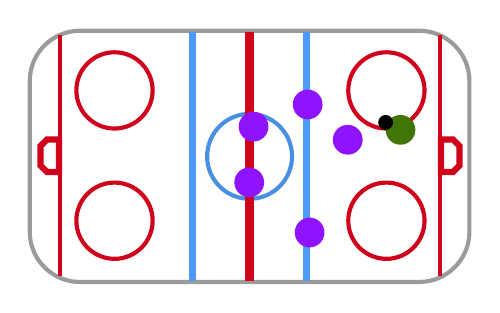
\begin{tikzpicture}[x=0.75pt,y=0.75pt,yscale=-1,xscale=1]
%uncomment if require: \path (0,142.66665649414062); %set diagram left start at 0, and has height of 142.66665649414062

%Rounded Rect [id:dp6258107511117066] 
\draw  [color={rgb, 255:red, 155; green, 155; blue, 155 }  ,draw opacity=1 ][fill={rgb, 255:red, 255; green, 255; blue, 255 }  ,fill opacity=1 ][line width=1.5]  (17,34.16) .. controls (17,20.79) and (27.84,9.95) .. (41.21,9.95) -- (204.62,9.95) .. controls (217.99,9.95) and (228.83,20.79) .. (228.83,34.16) -- (228.83,106.79) .. controls (228.83,120.16) and (217.99,131) .. (204.62,131) -- (41.21,131) .. controls (27.84,131) and (17,120.16) .. (17,106.79) -- cycle ;
%Shape: Circle [id:dp3018457504446248] 
\draw  [color={rgb, 255:red, 74; green, 144; blue, 226 }  ,draw opacity=1 ][line width=1.5]  (102.46,70.48) .. controls (102.46,59.18) and (111.62,50.02) .. (122.92,50.02) .. controls (134.22,50.02) and (143.37,59.18) .. (143.37,70.48) .. controls (143.37,81.78) and (134.22,90.93) .. (122.92,90.93) .. controls (111.62,90.93) and (102.46,81.78) .. (102.46,70.48) -- cycle ;
%Shape: Ellipse [id:dp07466971800950373] 
\draw  [color={rgb, 255:red, 208; green, 2; blue, 27 }  ,draw opacity=1 ][line width=1.5]  (39.46,38.7) .. controls (39.46,28.56) and (47.68,20.33) .. (57.83,20.33) .. controls (67.97,20.33) and (76.2,28.56) .. (76.2,38.7) .. controls (76.2,48.85) and (67.97,57.07) .. (57.83,57.07) .. controls (47.68,57.07) and (39.46,48.85) .. (39.46,38.7) -- cycle ;
%Shape: Circle [id:dp3308444073961254] 
\draw  [color={rgb, 255:red, 208; green, 2; blue, 27 }  ,draw opacity=1 ][line width=1.5]  (39.46,101.48) .. controls (39.46,91.34) and (47.68,83.11) .. (57.83,83.11) .. controls (67.97,83.11) and (76.2,91.34) .. (76.2,101.48) .. controls (76.2,111.63) and (67.97,119.85) .. (57.83,119.85) .. controls (47.68,119.85) and (39.46,111.63) .. (39.46,101.48) -- cycle ;
%Straight Lines [id:da4686331974076998] 
\draw [color={rgb, 255:red, 76; green, 154; blue, 249 }  ,draw opacity=1 ][line width=2.25]    (95.46,10.48) -- (95.46,130.48) ;


%Straight Lines [id:da11020079231172764] 
\draw [color={rgb, 255:red, 76; green, 154; blue, 249 }  ,draw opacity=1 ][line width=2.25]    (150.37,10.48) -- (150.37,130.48) ;


%Straight Lines [id:da2635334919770973] 
\draw [color={rgb, 255:red, 208; green, 2; blue, 27 }  ,draw opacity=1 ][line width=3]    (122.92,10.48) -- (122.92,130.48) ;


%Straight Lines [id:da6116270738771739] 
\draw [color={rgb, 255:red, 208; green, 2; blue, 27 }  ,draw opacity=1 ][line width=1.5]    (214.62,12) -- (214.62,128.33) ;


%Straight Lines [id:da07393178950615886] 
\draw [color={rgb, 255:red, 208; green, 2; blue, 27 }  ,draw opacity=1 ][line width=1.5]    (31.62,12) -- (31.62,128.33) ;


%Snip Same Side Corner Rect [id:dp04583555728641042] 
\draw  [color={rgb, 255:red, 208; green, 2; blue, 27 }  ,draw opacity=1 ][line width=2.25]  (220.96,62.35) -- (224.09,65.48) -- (224.09,74.85) -- (220.96,77.98) -- (215.16,77.98) -- (215.16,77.98) -- (215.16,62.35) -- (215.16,62.35) -- cycle ;
%Snip Same Side Corner Rect [id:dp8006864589098481] 
\draw  [color={rgb, 255:red, 208; green, 2; blue, 27 }  ,draw opacity=1 ][line width=2.25]  (25.28,77.98) -- (22.16,74.85) -- (22.16,65.48) -- (25.28,62.35) -- (31.09,62.35) -- (31.09,62.35) -- (31.09,77.98) -- (31.09,77.98) -- cycle ;
%Shape: Ellipse [id:dp2585703755974025] 
\draw  [color={rgb, 255:red, 208; green, 2; blue, 27 }  ,draw opacity=1 ][line width=1.5]  (170.46,38.7) .. controls (170.46,28.56) and (178.68,20.33) .. (188.83,20.33) .. controls (198.97,20.33) and (207.2,28.56) .. (207.2,38.7) .. controls (207.2,48.85) and (198.97,57.07) .. (188.83,57.07) .. controls (178.68,57.07) and (170.46,48.85) .. (170.46,38.7) -- cycle ;
%Shape: Circle [id:dp6471986972737049] 
\draw  [color={rgb, 255:red, 208; green, 2; blue, 27 }  ,draw opacity=1 ][line width=1.5]  (170.46,101.48) .. controls (170.46,91.34) and (178.68,83.11) .. (188.83,83.11) .. controls (198.97,83.11) and (207.2,91.34) .. (207.2,101.48) .. controls (207.2,111.63) and (198.97,119.85) .. (188.83,119.85) .. controls (178.68,119.85) and (170.46,111.63) .. (170.46,101.48) -- cycle ;

%Shape: Circle [id:dp22961674506792207] 
\draw  [draw opacity=0][fill={rgb, 255:red, 144; green, 19; blue, 254 }  ,fill opacity=1 ] (117.67,56.17) .. controls (117.67,52.21) and (120.88,49) .. (124.83,49) .. controls (128.79,49) and (132,52.21) .. (132,56.17) .. controls (132,60.12) and (128.79,63.33) .. (124.83,63.33) .. controls (120.88,63.33) and (117.67,60.12) .. (117.67,56.17) -- cycle ;
%Shape: Circle [id:dp361708851528006] 
\draw  [draw opacity=0][fill={rgb, 255:red, 144; green, 19; blue, 254 }  ,fill opacity=1 ] (144.67,107.17) .. controls (144.67,103.21) and (147.88,100) .. (151.83,100) .. controls (155.79,100) and (159,103.21) .. (159,107.17) .. controls (159,111.12) and (155.79,114.33) .. (151.83,114.33) .. controls (147.88,114.33) and (144.67,111.12) .. (144.67,107.17) -- cycle ;
%Shape: Circle [id:dp9538471188856912] 
\draw  [draw opacity=0][fill={rgb, 255:red, 144; green, 19; blue, 254 }  ,fill opacity=1 ] (163.04,62.48) .. controls (163.04,58.52) and (166.25,55.31) .. (170.21,55.31) .. controls (174.17,55.31) and (177.37,58.52) .. (177.37,62.48) .. controls (177.37,66.43) and (174.17,69.64) .. (170.21,69.64) .. controls (166.25,69.64) and (163.04,66.43) .. (163.04,62.48) -- cycle ;
%Shape: Circle [id:dp742379199123014] 
\draw  [draw opacity=0][fill={rgb, 255:red, 144; green, 19; blue, 254 }  ,fill opacity=1 ] (115.58,83.02) .. controls (115.58,79.06) and (118.79,75.85) .. (122.75,75.85) .. controls (126.71,75.85) and (129.92,79.06) .. (129.92,83.02) .. controls (129.92,86.98) and (126.71,90.18) .. (122.75,90.18) .. controls (118.79,90.18) and (115.58,86.98) .. (115.58,83.02) -- cycle ;
%Shape: Circle [id:dp7930588131530469] 
\draw  [draw opacity=0][fill={rgb, 255:red, 144; green, 19; blue, 254 }  ,fill opacity=1 ] (143.75,45.48) .. controls (143.75,41.52) and (146.96,38.31) .. (150.92,38.31) .. controls (154.87,38.31) and (158.08,41.52) .. (158.08,45.48) .. controls (158.08,49.43) and (154.87,52.64) .. (150.92,52.64) .. controls (146.96,52.64) and (143.75,49.43) .. (143.75,45.48) -- cycle ;
%Shape: Circle [id:dp049628433650009685] 
\draw  [draw opacity=0][fill={rgb, 255:red, 65; green, 117; blue, 5 }  ,fill opacity=1 ] (188.46,57.7) .. controls (188.46,53.74) and (191.67,50.54) .. (195.62,50.54) .. controls (199.58,50.54) and (202.79,53.74) .. (202.79,57.7) .. controls (202.79,61.66) and (199.58,64.87) .. (195.62,64.87) .. controls (191.67,64.87) and (188.46,61.66) .. (188.46,57.7) -- cycle ;
%Shape: Circle [id:dp3200961501093873] 
\draw  [draw opacity=0][fill={rgb, 255:red, 0; green, 0; blue, 0 }  ,fill opacity=1 ] (184.88,54.12) .. controls (184.88,52.14) and (186.48,50.54) .. (188.46,50.54) .. controls (190.44,50.54) and (192.04,52.14) .. (192.04,54.12) .. controls (192.04,56.1) and (190.44,57.7) .. (188.46,57.7) .. controls (186.48,57.7) and (184.88,56.1) .. (184.88,54.12) -- cycle ;




\end{tikzpicture}

\end{minipage}

\begin{distributions}[Trap/Forecheck slider]
Affects whether team's more likely to follow \textbf{Forecheck} or \textbf{Neutral Zone} strategies.
\begin{itemize}
	\item	If more neutral zone, then may start setting up there while the opponent is still in their zone.
	\item	Then, they'll sit there while nothing happens.
	\item	Probably better \textcolor{teal}{to max}, or almost max, the slider.
\end{itemize}
\end{distributions}

\subsection*{Offensive Pressure}
Determines how aggressive or passive you want your players to be while in the \textbf{offensive zone}.

Both aggressive and full attack are more about the \textbf{defenders}:

\paragraph{Full Attack} Best for when your team is trailing and you need to get some offense going, particularly late in the third period.

\begin{itemize}[leftmargin = *]
	\item	Means defenders will pretty much always get in on the play.
\end{itemize}

\paragraph{Aggressive}: 

\begin{itemize}[leftmargin = *]
	\item	Means defenders will sometimes get in on the play.
	\item	Second most aggressive setting.
	\item	Defenders will look to jump into the offense more frequently, but will still keep their defensive duties in mind.
\end{itemize}

\paragraph{Conservative}: 

\begin{itemize}[leftmargin = *]
	\item	Second most passive setting.
	\item	Basically defenders do what they're supposed to do and they'll try not to be in a bad position.
	\item	Defenders will sit back just in case the opposition retrieves the puck and starts an attack.
	\item	They will still occasionally jump into the play to generate offense.
\end{itemize}

\paragraph{\textcolor{teal}{Defend Lead}} Good setting for the third period when you're protecting a lead. 

\begin{itemize}[leftmargin = *]
	\item	Most passive setting.
	\item	Defenders will be as cautious as possible.
	\item	Prevents a lot of breakaways from occurring.
\end{itemize}

\paragraph{Standard}: 

\begin{itemize}[leftmargin = *]
	\item	Most common setting.
	\item	Balance between aggressive and conservative offensive pressures.
\end{itemize}

\subsection*{Defensive Pressure}
Determines how aggressive or passive you want your players to be while in \textbf{your zone}.

\paragraph{Contain Puck}: 

\begin{itemize}[leftmargin = *]
	\item	Players are set up in front of the net.
	\item	Players are active closing down on the while looking to block shots.
\end{itemize}

\paragraph{Normal}: Good mix of man to man and zone coverage.

\begin{itemize}[leftmargin = *]
	\item	Players move towards the opposition players they are covering.
	\item	Other players stay close to the net to block shots.
\end{itemize}

\paragraph{\textcolor{teal}{High Pressure}}: 

\begin{itemize}[leftmargin = *]
	\item	Players chase down the puck carrier.
	\item	Aggressively trying to win control of the puck.
\end{itemize}

\paragraph{Protect Net}: 

\begin{itemize}[leftmargin = *]
	\item	Almost all of your players are set up in front of your goaltender to block incoming shots and clear away rebounds.
\end{itemize}

\paragraph{Puck Side Attack}: 

\begin{itemize}[leftmargin = *]
	\item	Players on the same side as the puck will put pressure on the puck carrier.
	\item	Other players will wait for the puck to move closer to their position to pressure the puck carrier.
\end{itemize}

\subsection*{Defensive Strategy}

\textcolor{teal}{Collapsing}

\paragraph{}: 

\begin{minipage}{0.4\columnwidth}
\begin{itemize}[leftmargin = *]
	\item	
\end{itemize}
\end{minipage}
\begin{minipage}{0.6\columnwidth}

\end{minipage}

\subsection*{Penalty Kill}

\textcolor{teal}{Passive Box}

\paragraph{}: 

\begin{minipage}{0.4\columnwidth}
\begin{itemize}[leftmargin = *]
	\item	
\end{itemize}
\end{minipage}
\begin{minipage}{0.6\columnwidth}

\end{minipage}

\subsection*{Powerplay}

\textcolor{teal}{Overload}

\paragraph{}: 

\begin{minipage}{0.4\columnwidth}
\begin{itemize}[leftmargin = *]
	\item	
\end{itemize}
\end{minipage}
\begin{minipage}{0.6\columnwidth}

\end{minipage}

\begin{distributions}[PP Carry/Dump]
\textcolor{teal}{minimum}
\end{distributions}

\subsection*{Control Breakout}

\textcolor{teal}{Three High}

\paragraph{}: 

\begin{minipage}{0.4\columnwidth}
\begin{itemize}[leftmargin = *]
	\item	
\end{itemize}
\end{minipage}
\begin{minipage}{0.6\columnwidth}

\end{minipage}

\subsection*{Power Play Breakout}

\textcolor{teal}{Carry Option}

\paragraph{}: 

\begin{minipage}{0.4\columnwidth}
\begin{itemize}[leftmargin = *]
	\item	
\end{itemize}
\end{minipage}
\begin{minipage}{0.6\columnwidth}

\end{minipage}

\subsection*{Quick Breakout}

\textcolor{teal}{Leave Zone Early}

\paragraph{}: 

\begin{minipage}{0.4\columnwidth}
\begin{itemize}[leftmargin = *]
	\item	
\end{itemize}
\end{minipage}
\begin{minipage}{0.6\columnwidth}

\end{minipage}


\end{multicols*}
%% -----------------------------
%% Fin du document
%% -----------------------------
\end{document}
